\documentclass[danish ,a4paper,12pt]{article}
\usepackage[utf8]{inputenc}
\usepackage[table]{xcolor}% http://ctan.org/pkg/xcolor
\title{Bachelor projekt}
\author{msan18 }
\date{Juni 2021}

\usepackage{booktabs}
\usepackage{multirow}
\usepackage{rotating}
\usepackage{soul}
\usepackage[utf8]{inputenc}
%\usepackage[english]{babel}
\usepackage{apacite}
\usepackage[square,numbers]{natbib}
\bibliographystyle{apacite}
\usepackage{import}


%Title and author
\title{Bibliography management: \texttt{natbib} package}
\author{overleaf}
\date{}
\usepackage{amsmath}
\usepackage{wrapfig}
\usepackage{amsfonts}
\usepackage{amssymb}
\usepackage{graphicx}
\setcitestyle{authoryear,open={(},close={)}}
\graphicspath{ {./images/} }
\usepackage{url}
\usepackage{csquotes}
\usepackage{fullpage}
\usepackage{tabularx}
\usepackage{dcolumn}
\usepackage{float}
\usepackage{caption}
\usepackage{makecell}
\renewcommand\theadfont{\bfseries}
\usepackage{threeparttable}
\usepackage[colorlinks=true, hypertexnames=true, linkcolor=black, citecolor=black, urlcolor=black]{hyperref}
\usepackage{pdflscape}
\usepackage{rotating}
\usepackage{dcolumn}
\usepackage{blkarray}
\usepackage{array}
\usepackage{eurosym}
\usepackage{longtable}
\usepackage[]{multirow}
\usepackage{csquotes}
\usepackage{epstopdf}
\usepackage{soul}
\usepackage{float}
\usepackage{rotfloat}
\usepackage{subcaption}
\usepackage{parskip}
\usepackage{enumitem}
\usepackage{placeins}
\usepackage{tikz}
\usepackage{listings}
\usepackage{setspace}




\usepackage[a4paper,margin=1in,headheight=.4in,headsep=12pt,heightrounded]{geometry}
\usepackage{fancyhdr}
\usetikzlibrary{arrows,automata,positioning, fit, calc}
\tikzset{
    state/.style={
           rectangle,
           rounded corners,
           draw=black, very thick,
           minimum height=2em,
           inner sep=4pt,
           text centered,
           },
}

\usepackage[T1]{fontenc}
%\usepackage[table,xcdraw]{xcolor}
\renewcommand{\figurename}{\textbf{Figure}}
\renewcommand{\tablename}{Table}

%\addto\captionsenglish{\renewcommand{\appendixname}{Appendiks}}
%\usepackage[title]{appendix}





\setlength\parindent{15pt}
\newcommand{\dd}[1]{\mathrm{d}#1}

\makeatletter
% make numeric styles use name format
\patchcmd{\NAT@test}{\else \NAT@nm}{\else \NAT@nmfmt{\NAT@nm}}{}{}
% define \citepos just like \citet
\DeclareRobustCommand\citepos
  {\begingroup
   \let\NAT@nmfmt\NAT@posfmt% ...except with a different name format
   \NAT@swafalse\let\NAT@ctype\z@\NAT@partrue
   \@ifstar{\NAT@fulltrue\NAT@citetp}{\NAT@fullfalse\NAT@citetp}}
\let\NAT@orig@nmfmt\NAT@nmfmt
\def\NAT@posfmt#1{\NAT@orig@nmfmt{#1's}}
\makeatother
\raggedbottom
\usepackage{ragged2e}
\definecolor{numbercolor}{gray}{0.7}		% Definerer en farve til brug til kapiteludseende



\pagestyle{headings}


\pagestyle{fancy}
\fancyhf{}
\rhead{Københavns Universitet}
\fancyhead[LE]{\nouppercase{\rightmark}}
\rfoot{Page \thepage}

\patchcmd{\maketitle}{\@fnsymbol}{\@arabic}{}{}
% \patchcmd{\maketitle}{\setcounter{footnote}{0}}{}{}{}
\makeatother

\makeatletter
\pgfdeclaregenericanchor{top base}{%
  \csname pgf@anchor@#1@north\endcsname
  \pgf@anchor@generic@top@base@main
}
\pgfdeclaregenericanchor{top base west}{%
  \csname pgf@anchor@#1@north west\endcsname
  \pgf@anchor@generic@top@base@main
}
\pgfdeclaregenericanchor{top base east}{%
  \csname pgf@anchor@#1@north east\endcsname
  \pgf@anchor@generic@top@base@main
}
\def\pgf@anchor@generic@top@base@main{%
  {%
    \pgfmathsetlength\pgf@ya{\pgfkeysvalueof{/pgf/outer ysep}}%
    \advance\pgf@y-\pgf@ya
    \pgfmathsetlength\pgf@ya{\pgfkeysvalueof{/pgf/inner ysep}}%
    \advance\pgf@y-\pgf@ya
    \pgf@ya=0pt
    \pgfutil@loop
    \ifdim\pgf@y>\baselineskip
      \advance\pgf@y-\baselineskip
      \advance\pgf@ya\baselineskip
    \pgfutil@repeat
    \global\pgf@y=\pgf@ya
  }%
}
\makeatother

\usepackage{setspace}

  \renewcommand{\contentsname}
    {Indholdsfortegnelse}
  \renewcommand{\listfigurename}{Liste af figurer}
  \renewcommand{\listtablename}{Liste af tabeller}

  \usepackage{array}
\newcolumntype{L}[1]{>{\raggedright\let\newline\\\arraybackslash\hspace{0pt}}m{#1}}
\newcolumntype{C}[1]{>{\centering\let\newline\\\arraybackslash\hspace{0pt}}m{#1}}
\newcolumntype{R}[1]{>{\raggedleft\let\newline\\\arraybackslash\hspace{0pt}}m{#1}}
 

\begin{document}

\rowcolors{2}{white}{gray!10}

\linespread{1.5}

\fancypagestyle{plain}{%
  \fancyhf{}%
  \fancyfoot[R]{ \thepage}%
  \renewcommand{\headrulewidth}{0pt}% Line at the header invisible
}
\frontmatter


\thispagestyle{empty}

\begin{titlepage}

\newcommand{\HRule}{\rule{\linewidth}{0.5mm}} % Defines a new command for the horizontal lines, change thickness here

\center % Center everything on the page
 
%----------------------------------------------------------------------------------------
%	HEADING SECTIONS
%----------------------------------------------------------------------------------------

\textsc{\LARGE University of Copenhagen}\\[1.5cm] % Name of your university/college
% Major heading such as course name
%\textsc{\large Assignment 1}\\[0.5cm] % Minor heading such as course title

%----------------------------------------------------------------------------------------
%	TITLE SECTION
%----------------------------------------------------------------------------------------

\HRule \\[0.4cm]
\textsc{\Large Master Thesis}\\[0.5cm] 
{ \huge \bfseries Management}\\[0.4cm] % Title of your document
\textsc{\Large Spring 2023}\\[0.5cm] 
\HRule \\[1.5cm]
 
%----------------------------------------------------------------------------------------
%	AUTHOR SECTION
%----------------------------------------------------------------------------------------

\begin{minipage}{0.4\textwidth}
\begin{flushleft} \large
\emph{Author:}\\
Martin Skafte Andersen \\ TGX333 \\
\end{flushleft}
\end{minipage}
~
\begin{minipage}{0.4\textwidth}
\begin{flushright} \large
\emph{Supervisor:} \\
Stefan Voigt \\
\end{flushright}
\end{minipage}\\[5cm]
%----------------------------------------------------------------------------------------
%	DATE SECTION
%----------------------------------------------------------------------------------------
\begin{flushleft}
    
{\large Submitted: December 20, 2022}\\ % Date, change the \today to a set date if you want to be precise
{\large ECTS: 7.5}\\
{\large Characters: 35.900 of 36.000}\\[2cm]
\end{flushleft}
%----------------------------------------------------------------------------------------
%	LOGO SECTION
%----------------------------------------------------------------------------------------

%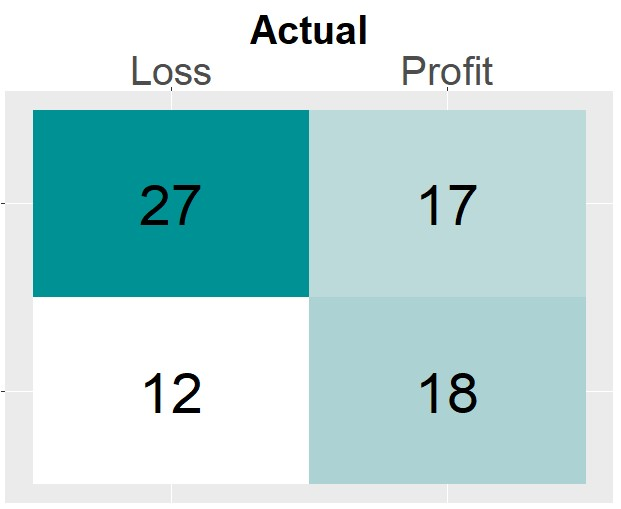
\includegraphics[width=50px, keepaspectratio]{Projekt/Figures/conf_mat_mom.jpg}\\[1cm] % Include a department/university logo - this will require the graphicx package
 
%----------------------------------------------------------------------------------------

\vfill % Fill the rest of the page with whitespace

\end{titlepage}


%%%% Indholdsfortegnelse (TOC) %%%%

\phantomsection													% Kunstigt afsnit, som hyperlinks kan 'holde fast i'
\pdfbookmark[0]{Indholdsfortegnelse}{indhold}					% Tildeler en klikbar bookmark til den endelige PDF
\tableofcontents*	
\newpage
% Here we can add figures and tables
%\listoffigures
%\newpage
%\listoftables
% Indholdsfortegnelsen (kaldet ToC) 

%\addtocontents{toc}{\protect\newpage}							% Fremtvinger sideskift i ToC hvis noedvendig (der hvor koden placeres)

\renewcommand{\cleardoublepage}{\newpage}
\mainmatter

\fancypagestyle{plain}{%
  \fancyhf{}%
  \fancyfoot[R]{Side \thepage}%
  \renewcommand{\headrulewidth}{0pt}% Line at the header invisible
}

\vspace{1.5 cm}
\selectfont



\section{Introduction} \label{sec:intro}
The global financial markets has experienced tremendous growth within sustainable investing. The mega-trend has evolved over the last two decades and incorporates an approach that emphasises corporate focus on non-financial information categorized as environmental, social, and governance (ESG) in portfolio selection. A growing societal focus on capital allocation toward sustainable investments, accountability and transparency, implies that firms cannot override infringement cases such as oil spills, accounting fraud and the use of child labor, which formerly have experienced less public attention. Furthermore, the research focus on climate change has enlightened the public and assisted a cultural shift toward a stronger focus on ESG. The escalation in sustainable investing has been institutionalized through the United Nations Principle for Responsible Investments (PRI). The PRI's long term ambition is to develop a more sustainable global financial system by encouraging and supporting signatories in incorporating the ESG factors into investment decisions. By participating in the treaty, asset managers commit to implement the financial and reporting principles for sustainable investments. The treaty has increased its number of signatories from 100 in 2006 with USD 6 trillion in assets under management (AUM) to 5.179 signatories with more than USD 121 trillion AUM \footnote{//www.unpri.org/pri.}. 

ESG objectives are becoming a primary target in asset management, where reallocation of capital has large complications for financial decision making and asset pricing. In line with increasing focus on sustainable investing, the CEO of one of the world largest asset manager, BlackRock, Larry Fink wrote in his 2020 annual letter to CEO's that his firm would exit "investments that present a high sustainability-related risk" \citep{Blackrock}. 

Understanding the relationship between SDG-related news and stock returns could provide valuable insights for investors who are looking to incorporate sustainability criteria into their investment decisions. This is particularly important as sustainable investing continues to grow in popularity, with more and more investors seeking to align their portfolios with their values. Additionally, understanding the relationship between SDG-related news and stock returns could also inform the efforts of companies and policymakers to achieve the SDGs by incentivizing companies to prioritize sustainability initiatives and enabling policymakers to design policies that support sustainable development. Therefore, investigating the relationship between SDG-related news and stock returns is not only important for investors, but also for companies, policymakers, and society as a whole.


- Massive inflow to sustainability funds
- Increased academic focus
- missing clear link
- ESG --> lower expected returns and thus a premium for sin stocks
- Some find ESG --> greater returns


- ESG ratings --> low frequency/granularity --> more difficult to use as a indicator
- ESG rating --> doesn't change very often, so difficult to use as explaining variable for returns


The growing attention towards sustainability in general has increased the focus on company specific ESG-ratings. However, ESG profiles can be difficult to

The main disadvantage of earlier research are the samples behind the results. First, the samples are often small. Second, they consist of a fixed database of news articles, which mean that they cannot be used on a daily or monthly basis to actively manage a portfolio. This thesis utilizes a database that updates on a daily basis, indicating that all new events can be captured on a daily basis.


\subsection{Motivation}

\subsection{Problem statement}

As investors increasingly consider environmental, social, and governance (ESG) factors when making investment decisions, it is important to understand the relationship between ESG-related news and stock market returns.  Specifically, does news related to the United Nations' Sustainable Development Goals (SDGs) have an impact on firms' short-term and long-term market values. The overall research questions that this thesis will investigate is the following: \\

What is the relationship between news related to the United Nations' Sustainable Development Goals and stock market returns?

To investigate this question, I have developed two main hypotheses. First, I hypothesize that news related to SDGs does not have a significant short term impact on firms' market values. The hypothesis is partitioned between positive and negative news through creation of an "a" and a "b" hypothesis.  \\

\textbf{Hypothesis 1:} 

\begin{itemize}
  \item \textbf{a.}  Negative news related to the SDGs does not have a short term impact on firm's market values.
  \item \textbf{b.}  Positive news related to the SDGs does not have a short term impact on firm's market values.
\end{itemize}

Second, I hypothesize that news related to SDGs does not have a significant long-term impact on firms' market values. \\

\textbf{
Hypothesis 2: \textit{Positive and negative news related to the SDGs does not have a long term impact on firms' market values.}}

\begin{itemize}
  \item \textbf{a.}  Negative news related to the SDGs does not have a long term impact on firm's market values.
  \item \textbf{b.}  Positive news related to the SDGs does not have a long term impact on firm's market values.
\end{itemize}


By testing these hypotheses, I hope to contribute to a better understanding of the relationship between sustainability and financial performance. 

However, I also recognize that there may be factors that influence the relationship between SDG-related news and market values. 
To explore these potential moderators, I have developed two additional sub-questions, which ultimately should expand our interpretation of the results from the main hypotheses. 

One potential moderator is the specific SDG that the news is related to. Each of the 17 SDGs represents a different aspect of sustainable development, from eradicating poverty to ensuring access to clean water and sanitation. In this regard, I will review whether the potential impact of SDG-related news on short and long term market values is independent of which specific SDG the news are related to.

Another potential moderator is the firm's level of ESG risk. ESG risk refers to the degree to which a company's operations and business practices are aligned with environmental, social, and governance principles.
By splitting the analysis on the basis of firms' ESG risk profile, I can investigate whether the impact of SDG-related news on short and long term market values is dependent on the level of ESG risk of the company. 

 
By testing these hypotheses and exploring potential moderators, I hope to gain a more nuanced understanding of how SDG-related news may impact firms' market values. Moreover, this knowledge can help investors make more informed decisions around ESG investing and encourage companies to align their business practices with sustainable development principles.


%Hypothesis 1: \textit{Negative news related to the SDGs does not have a short term impact on firm' market value.}
%Hypothesis 1a: \textit{A potential impact is independent on which SDG the news are related to.}  
%Hypothesis 1b: \textit{The potential impact is independent on the firm's level of ESG risk.}

%Hypothesis 2: \textit{Positive news related to the SDGs does not have a short term impact on firm' market value.}
%Hypothesis 2a: \textit{A potential impact is independent on which SDG the news are related to.}  
%Hypothesis 2b: \textit{The potential impact is independent on the firm's level of ESG risk.}

%Hypothesis 3: \textit{The short term impact of news related to SDGs on firms' market value is equivalent for negative news and positive news.}

%Hypothesis 4: \textit{Negative news related to the SDGs does not have a long term effect on firms market value}
%Hypothesis 4a: \textit{The potential impact is independent on the firm's level of ESG risk.}


%Hypothesis 5: \textit{Positive news related to the SDGs does not have a long term effect on firms market value.}
%Hypothesis 5a: \textit{The potential impact is independent on the firm's level of ESG risk.} 

%Hypothesis 6: \textit{The long term impact of news related to SDGs on firms' market value is equivalent for negative news and positive news.}

\subsection{Method}

\subsection{Scope and delimitation}

\subsection{Structure}


\section{Literature review} \label{lit_rev}


\subsection{A short overview of ESG and Corporate Financial Performance}

The initial mentioning of the term "ESG" has been attributed to the study "Who Cares Wins"  by the UN Global Compact in 2004 \citep{WhoCaresWins}, where the succeeding "Who Cares Wins Initiative" from 2004-2008 was built on the idea of a all-win situation for the financial industry, society and the environment. The main purpose was to incentivize the financial industry to incorporate ESG topics into their financial decision-making. The initiative was successful as the aforementioned PRI was established few years later, after which the focus sustainability in the financial world has experienced a dramatic increase. In line with the increased funding and awareness to ESG in the financial industry, the academic attention towards the issues has evolved positively as well.
According to a 1970's essay by Friedman \citeyear{friedman2007} the sole responsibility of a firm is to generate profits for its shareholders. Such a view would imply that any ESG related activity, that is not a part of the core business, should not be taken forward by the manager and neither should investors integrate information on ESG into their financial decision making.

The recent literature seems to disagree whether investing in ESG-leaders generate over-performance (alpha) in terms of returns relative to ESG-laggards. Most literature acknowledge a certain investor response to ESG initiatives, which affects the stock price, but there seems to be no clear consensus on whether the relative performance is positive, negative or simply explainable by other factors. 

\cite{ESG_meta_analysis} made an meta-analysis of more than 2.000 studies looking into the potential of ESG investing. The results of the studies differ depending on which ESG methodology (e.g. source and granularity) were used and which financial metrics were applied (e.g. return or exposure to Fama-French factors). They conclude that the majority of studies find stable positive ESG impact on performance over time. However,  once screened for portfolio performance, such as transaction costs, the studies reporting a positive correlation decreases. 


Although the evidence of negative correlation between ESG-activities and CFP is limited, the theoretical foundation is supported by the aforementioned statement from Friedman and the efficient market hypothesis. If the market is partly driven by socially responsible investors that screen out low-ESG assets, then one would theoretically observe negative correlation between sustainable investments and CFP, and investors would pay a premium for their preference for sustainability. 


Some empirical studies give reason to doubt an optimistic view on a firm's ESG activities, providing evidence for financial costs for companies from being proactive in ESG matters. 

For example \cite{ESG_Frontier} integrates ESG characteristics in the portfolio construction of the efficient frontier instead of as a screening factor. They quantify the cost of ESG preferences as the drop in Sharpe ratio when choosing a portfolio with better ESG characteristics than the efficient portfolio. The authors find that integrating the ESG preferences by a proxy for governance, the maximum Sharpe ratio is achieved for a high level of ESG, implying that ethical goals can be done at little cost. Imposing constraints will always reduce the Sharpe ratio for any given ESG score. The proxies for E, S and overall ESG are weaker predictors of future profits. 

Moreover, the findings from \citep{uk_ESG_stock} show that companies with higher social performance scores exhibit minor returns than those with lower social performance scores. They state that social performance indicators are negatively related to stock returns and that abnormal returns are available from holding a portfolio of the socially least desirable firms. In addition, \cite{Kacperczyk_sin_stocks} advocate that so called "sin stocks"\footnote{Classified as companies involved in alcohol, tobacco, gambling or the weapons industry. } have higher expected returns than stocks of otherwise comparable characteristics, due to them being neglected by constrained investors. Negative screening will lead to these stocks being under-priced in relation to fundamental value.   

For example, using yearly sustainability ratings \cite{Shrunk_ESG_ALPHA} address the question whether non-financial information in ESG scores offers additional performance benefits by construct long-short ESG strategies and asses their value-added to investors. They find that claims of ESG out-performance only hold when considering isolated returns. However, when applying standard risk adjustments, the strategies perform like simple quality strategies constructed from accounting ratios. 


Supporting the evidence from \cite{ESG_meta_analysis}, the paper from \cite{factor_ESG_integration} investigates the impact of ESG integration on different factor-investment strategies. Their results show that a manager of a factor portfolio can increase the portfolio exposure towards ESG intensive companies without impairing the exposure toward the desired factors, such as value and low volatility. For example, the minimum volatility strategy only experienced a 7\% reduction in factor exposure from a 30\% increase in exposure to ESG. The results suggest that investors would be able to improve the ESG characteristics of their portfolio without harming their ability to capture market returns. 

Similarly \cite{ESG_exposure_approach} finds averagely positive ESG return premia between 2009 and 2020. They utilize an exposure-matching approach to isolate and measure the return premium related to ESG by neutralizing the exposure to other factors. The benefit is that they are able to control for risk and sector differences to measure month-on-month ESG returns. They also discuss the advantages of using their approach over a regression approach that sorts stocks into portfolios given ESG attributes, but mainly state that it is of more practical use whereas the latter is more useful within academia.

Additional research acknowledge an investor response to firm's ESG activities which affects the companies performance in different ways (\cite{lins2017social}; \cite{kim2014corporate}; \cite{el2011does}). These studies use yearly observations and explain their findings by concepts of trust-building in sustainable activities, which facilitates the firm to obtain benefits such as lower cost-of-capital, lower crash risk, higher and long-run profitability.

The insights from these findings dictate various long-term benefits of both investors and firms from engaging in ESG intensive investment activities. It is relevant to assume that these benefits are particularly suitable for long term investors in diversified portfolios, whereas short term investment strategies will require information on a more granular basis than yearly ratings, when implementing ESG factors into their investment decision. Applying yearly observations ignores the changing landscape of the market, where news are spreading promptly over the internet. Moreover, the potentially impulsive behavior of a large group of speculators and retail investors, who might base their decisions on instant new information becoming available, as per \cite{black1986noise}. Capitalizing on the possibilities of looking beyond yearly data points may add more insights into whether investors incorporate ESG-related information into their financial decision making \citep{Sustainable_sentiment}. 

Increasing the granularity of observations can be done by relying on public news articles, with a focus on ESG-related matters, as a proxy for ESG engagement of companies. 

- Sustainable investing with ESG rating uncertainty

\subsection{Relevant sentiment analysis literature}


Our approach evolves around a popular core of literature that links public sentiment, through news articles, with financial performance on the stock market. Two of the early comprehensive publications are \cite{tetlock_sentiment} and \cite{baker_sentiment}. \citeauthor{tetlock_sentiment} shows that high media pessimism predicts downward pressure on stock prices followed by a reversion to fundamentals. \citeauthor{baker_sentiment} studies how investor sentiment affects stock returns. Their main empirical finding is that future stock returns are conditional on beginning-of-period sentiment. That is, when sentiment is high, stocks that are attractive to speculators - small stocks, unprofitable stocks, high-volatility stocks and more - tend to earn relatively low subsequent returns, while if sentiment is low these stocks earn relatively high returns.   

\cite{Blancard_ESG_sentiment} utilize the ideas from the aforementioned authors to investigate the relationship between positive and negative ESG news and changes in firm market value. They conduct an event study and find that investors on average react negatively to negative events, while positive events has no impact. 

We want to elaborate on the relation between sustainability of firms and financial performance, by combining the ideas from the previous sections on ESG and sentiment analysis. We will focus on news articles that contain company specific information in relation to the United Nations Sustainable Development Goals\footnote{https://www.un.org/development/desa/disabilities/envision2030.html} (SDGs), and research how company valuation responds to such events. 



\subsection{Market theory}




\subsection{Identification of gap in the literature}



\section{Methodology and theory} \label{sec:method}
\subsection{The Event Study Methodology}

The short-term event study examine the behavior of stock returns around corporate events, and is used to measure shareholders' reaction to unexpected news. 
- Something with Fama


\subsection{The Market Adjusted Model}

In the context of event studies, an expected return model is a hypothetical prediction of the stock return. The individual stock price return is measured against the market return, as a simple way to control for potential effects of the event on the general market. The model does not adjust for basic CAPM risk and thus abstracts from the individual firm's distinct risk profile. The argument for implementing a simple model is to give a general overview of long and short term return-effects from events, and not to provide statistical conclusions. 
The daily excess returns are measured as the difference between the stock return and the market return on a given day, with the market return assumed to be the MXWO\footnote{https://www.msci.com/World} index:
\begin{equation}
    \text{Abnormal Returns} \:  (AR_{i,t}) = R_{i,t} - R_{M,t} 
\end{equation}
Where, $R_{i,t}$ is the return of stock \textit{i} on day \textit{t}, and $R_{M,t}$ is the return of the market on day \textit{t}. 

The returns series for stock \textit{i} is indexed wrt. the event date (t = 0) by setting the value to 100 and expressing the cumulative return of the future and foregoing observations with respect to this value, to isolate the effect of the event from the discrete trading days. 

The argument is that on t = 0 the information becomes available to the market. However, the investor will not be able to trade on the information before the following trading day. The return index is calculated as the 
cumulative product of the daily excess return leading up to or following the event date multiplied by 100. 

\subsection{Short-term abnormal returns}

The inspection of short-term abnormal return behavior covers (2n+1) trading days surrounding a corporate event: n days before to catch possible insiders information, the day of the event, and n days after. The short term analysis will use N = 10, which leaves a total window of 21 days [-10,+10] to investigate effect from an event. The effect of an event is expressed in terms of the abnormal return, defined as the difference between the realized ex-post return and the expected return, with the latter characterized as the expected return conditional on the event not taking place \citep{Event_studies}. Several models have been applied in the literature to estimate the short-term abnormal returns in event studies, which includes the CAPM, the Market Model, and multi-factor models. According to \cite{holler2014event} the most widely used is the Market Model, which assumes a linear relationship between the individual stock return and the market return. 

\subsubsection{The Market Model}

The Market Model is a single factor statistical model, which relates the return of a given security to the return of the market portfolio. The linear specification follows from the assumed joint normality of asset returns. For any given stock the model is defined as:

\begin{equation} \label{market_model}
    R_{i,t} = \alpha_i + \beta_i * R_{m,t} + \epsilon_{i,t},
\end{equation}
 where $R_{i,t}$ is the return of the stock \textit{i} on day \textit{t}, $\alpha_i$ is the regression intercept\footnote{The excess return of a stock relative to the market, that is not explained by the $\beta$.} for stock \textit{i}, $R_{m,t}$ is the market return on day \textit{t}, and
 $\beta_i$ is the sensitivity of $R_{i,t}$ to the market return.  

 The regression coefficients $\alpha_i$ and $\beta_i$ are computed as the stock returns of a given frequency on the market returns. To analyze the market participants' short-term reaction before and after the event date, the event window is set to +-10 days around the event date, and the estimation window of the regression is set to 120 days prior to the event, as proposed by \cite{Event_studies}. The linear ordinary least squares (OLS) has been applied in the estimation. \cite{brown1985using} investigate the properties of applying daily stock returns in event studies with the market model, and find that the model is well-specified under a variety of conditions. 

 With the expected returns predicted from the Market Model, the abnormal returns are defined as the residual between the realized and the expected returns for each event:
 \begin{equation}
     AR_{i,t} = R_{i,t} - (\alpha_i + \beta_i * R_{m,t})
 \end{equation}

 where $AR_{i,t}$ measures the shareholder's reaction to the event addressing firm \textit{i} at time \textit{t}  with $\alpha_i$ and $\beta_i$ defined as the OLS-parameter estimates from the regression in equation \ref{market_model}. The abnormal return can be transformed into average, cumulative, and cumulative average abnormal returns (for n = (1, ..., 10) by: 
  \begin{equation}
     AAR_t = \frac{1}{N} \sum_{i=1} ^{I} AR_i
 \end{equation}
 \begin{equation}
     CAR_{i,t}[-n,+n] = \sum_{\tau = t-n} ^{t+n} AR_{i,t}
 \end{equation}
 \begin{equation}
     CAAR_{[-n,+n]} = \sum_{\tau = t-n} ^{t+n} AR_{i,t}
 \end{equation}
 
 The AAR is the average of the AR per time period, the CAR is the cumulative sum of the AR per stock, and the CAAR is the cumulative sum of the AAR of all stocks and over windows. 



 

\subsection{Long-term abnormal returns}

\subsubsection{Portfolio sorts / Calendar Time Portfolio Approach}







\section{Empirical analysis} \label{sec:analysis}

\subsection{Data description}


\subsection{Estimation methodology}


\subsection{Abnormal returns and the Market Model}






\begin{figure}[!tbp]
  \centering
  \begin{minipage}[b]{0.45\textwidth}
    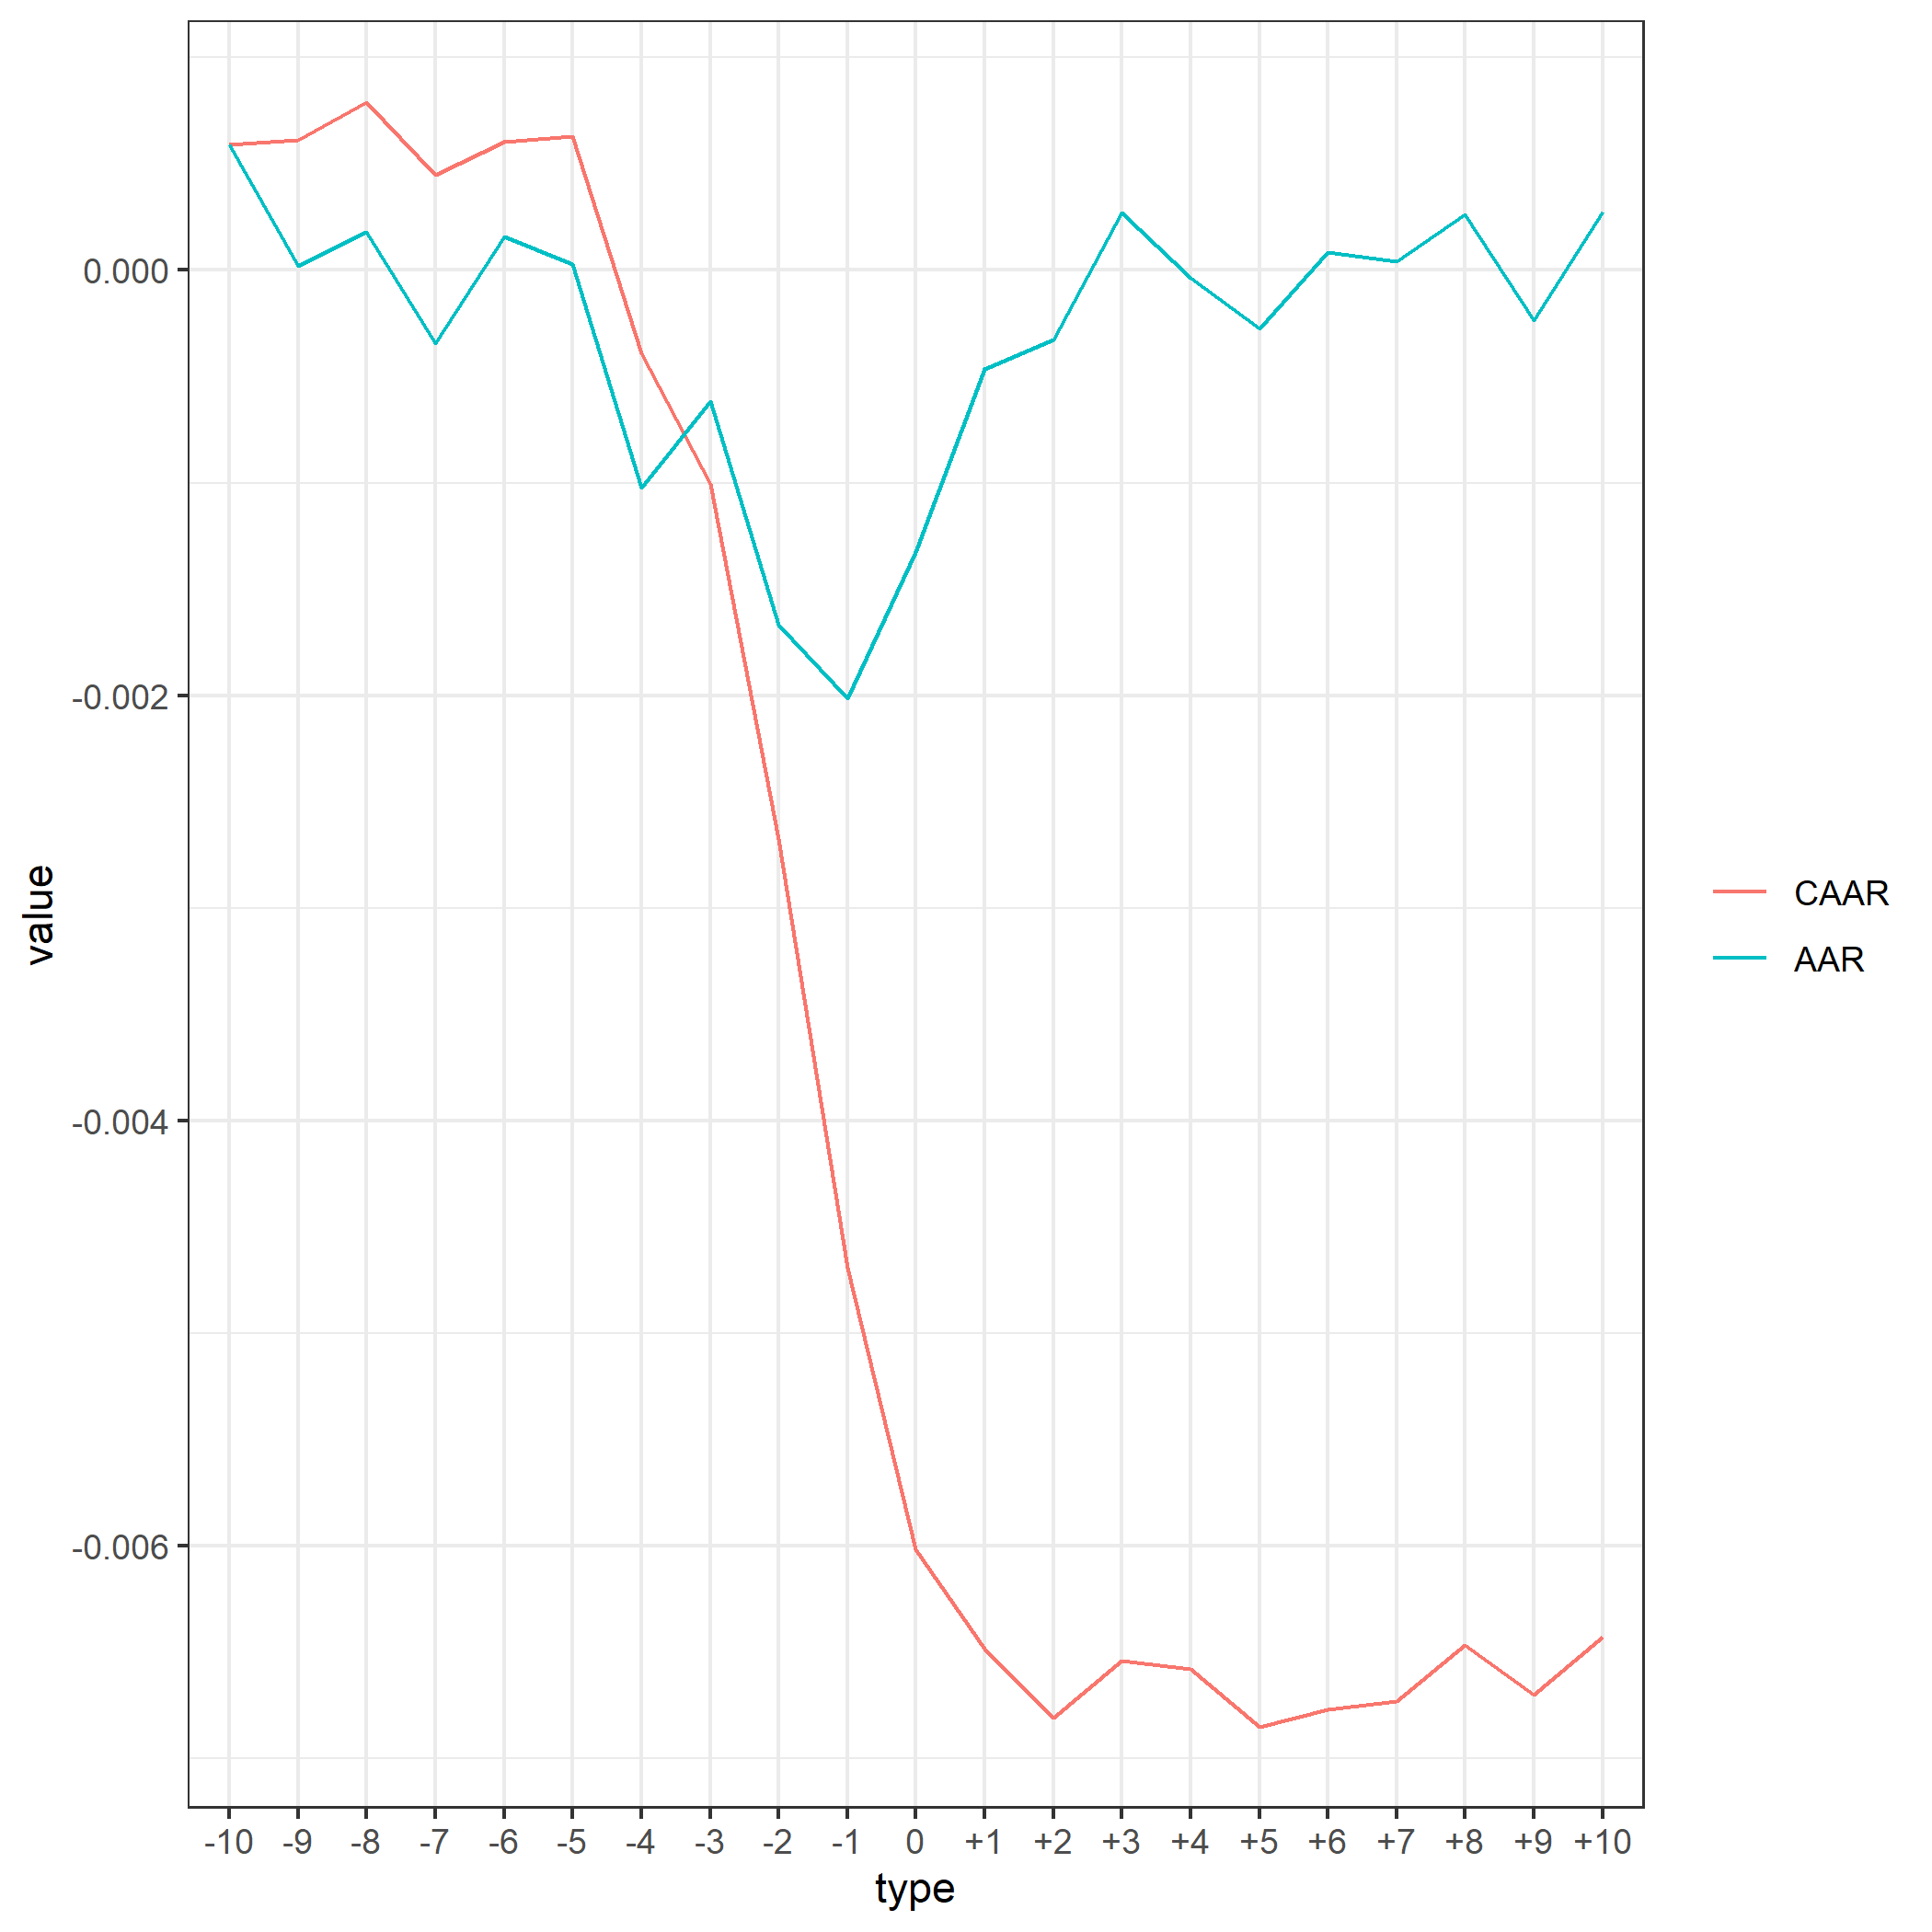
\includegraphics[scale=0.5]{Projekt/1.Figures analysis/ST_negative_all.png}
    \caption{Negative events}
  \end{minipage}
  \hfill
  \begin{minipage}[b]{0.45\textwidth}
    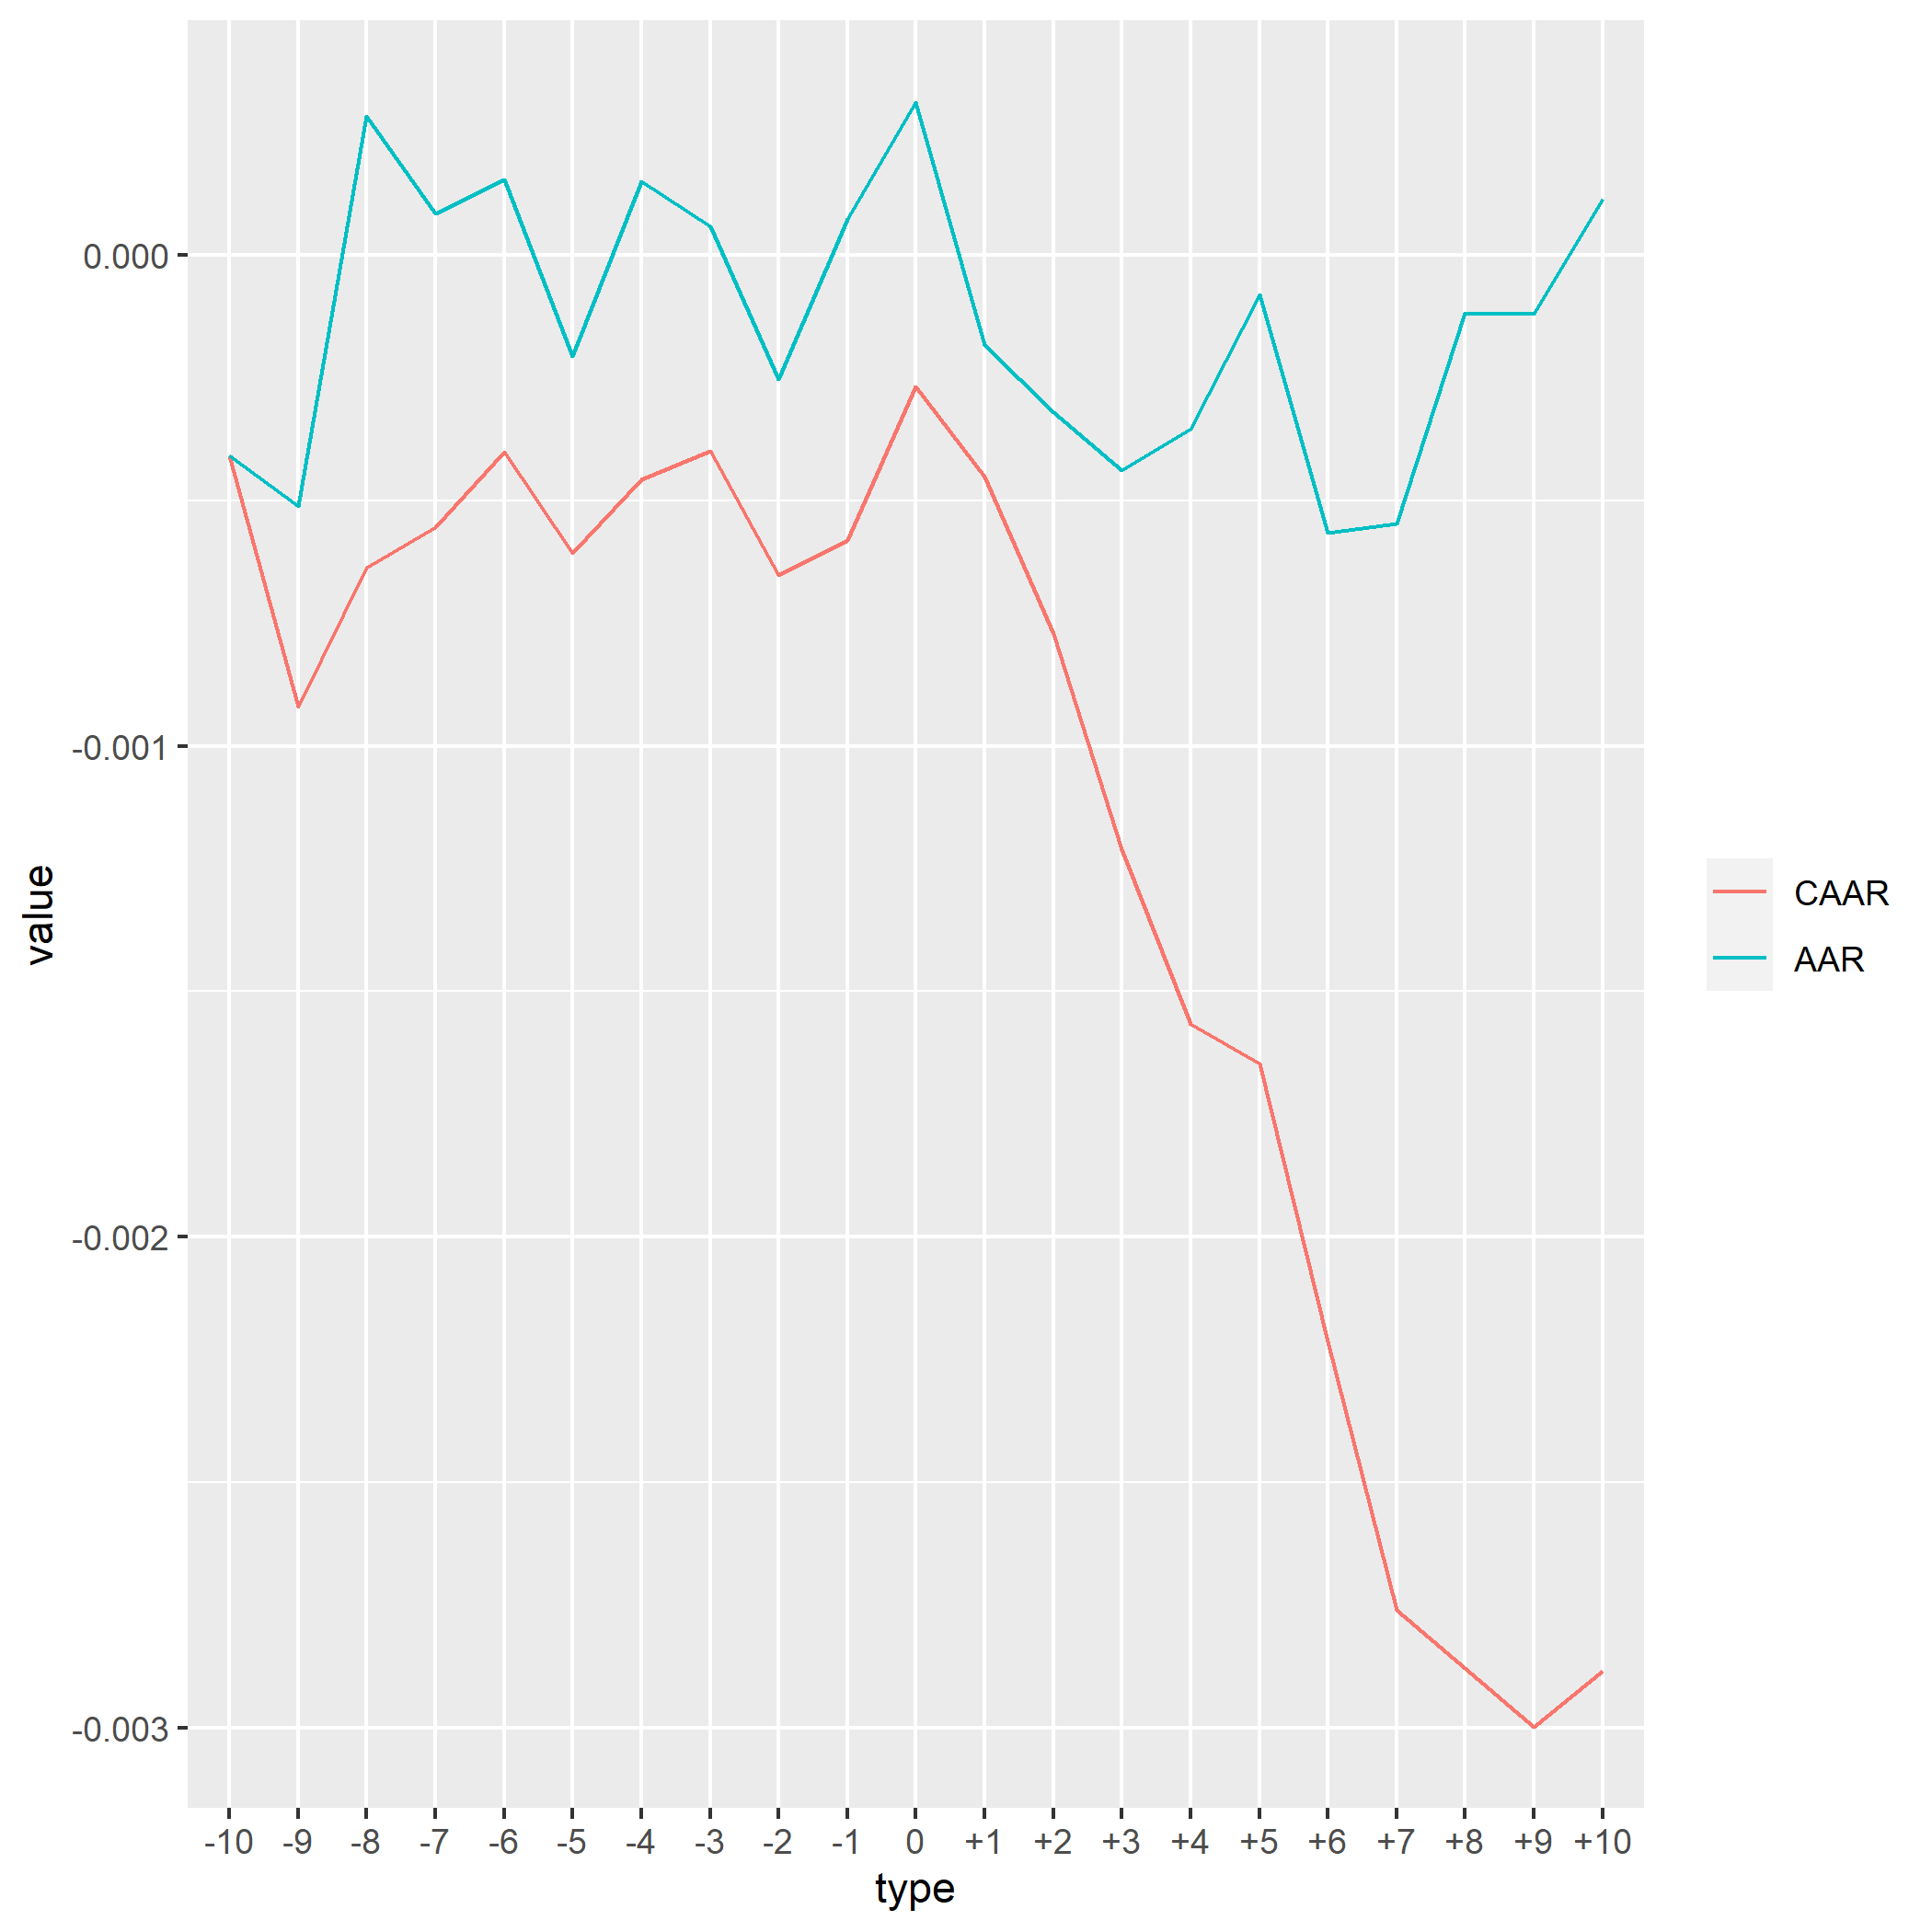
\includegraphics[scale=0.5]{Projekt/1.Figures analysis/ST_positive_all.png}
    \caption{Positive events}
  \end{minipage}
\end{figure}


\begin{figure}
    \centering
    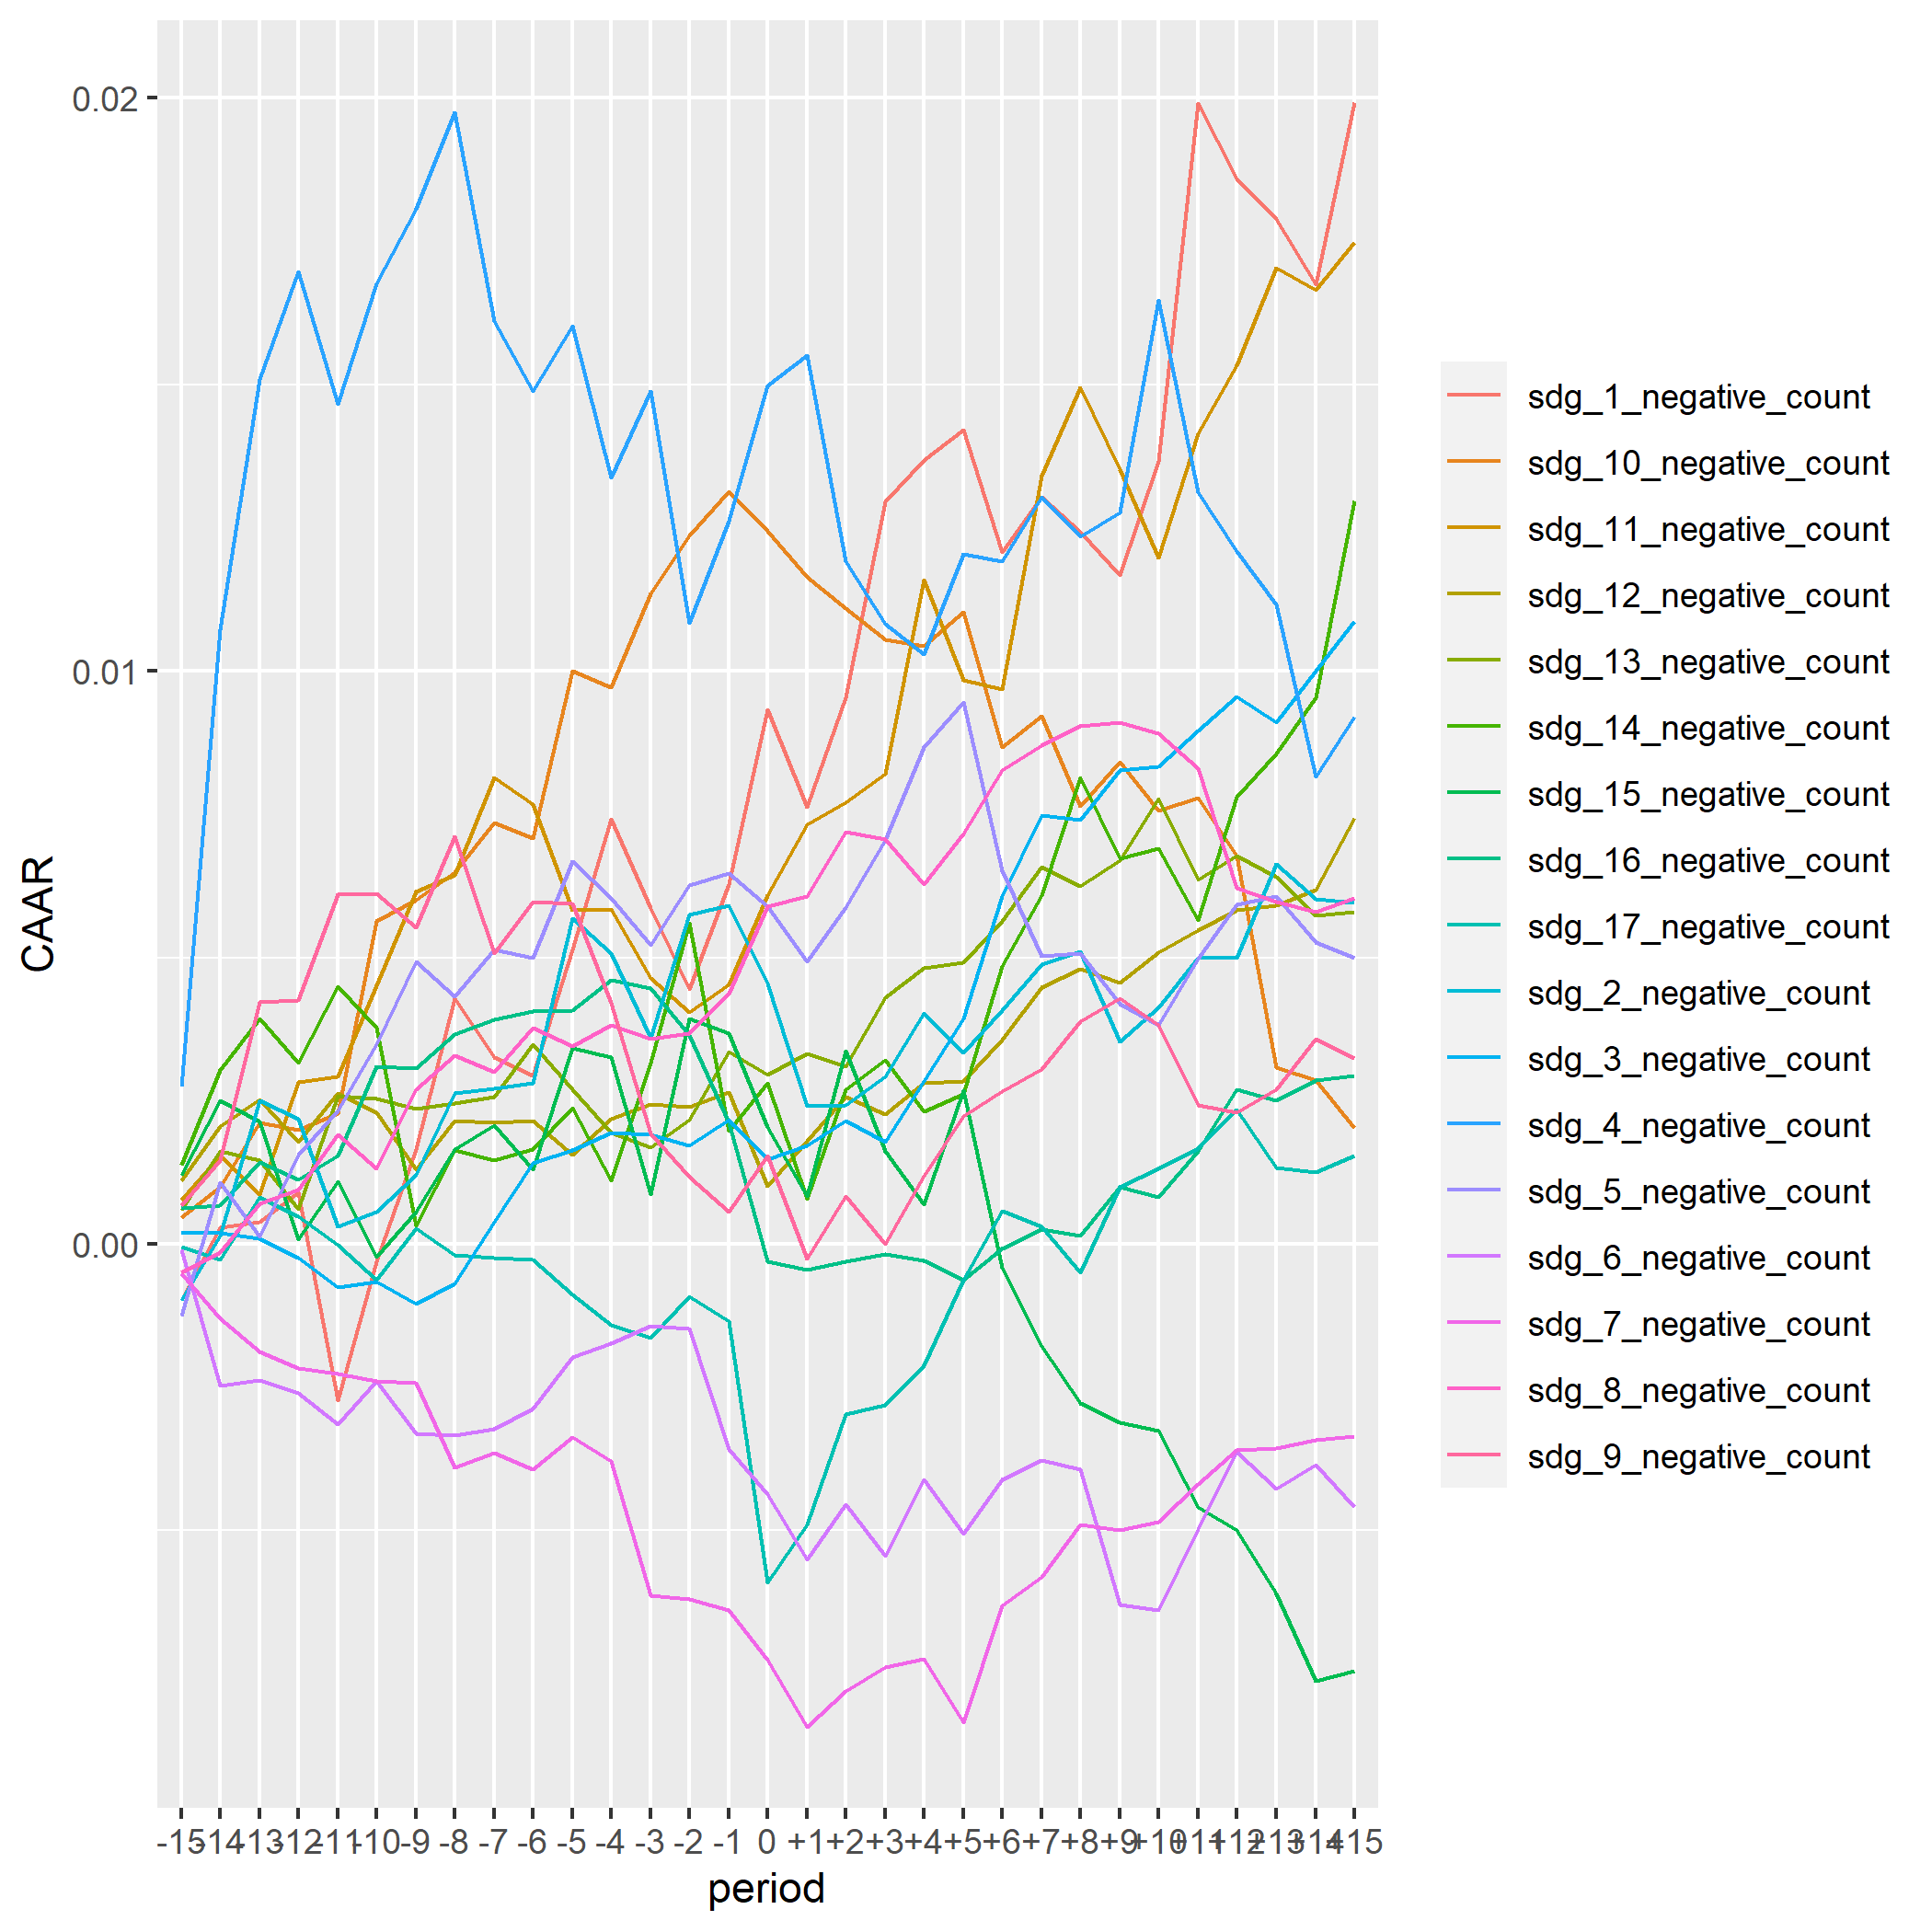
\includegraphics[scale=0.6]{Projekt/1.Figures analysis/ST_negative_sdgs.png}
    \caption{Short term positive news: AAR and CAAR}
    \label{fig:ST_pos_news}
\end{figure}

\section{Results} \label{results}
\input{Projekt/Results.tex}

\section{Discussion} \label{sec:discussion}
- To be able to actually trade this idea, we need a way of finding the negative events before they happen. 

- Future work could try to use the SDG signals (negative and positive events) as an indication of whether a company is expected to be downgraded, which there is some clear benefits in trading. I.e. refer to some paperps about this. 
\pagebreak

 \renewcommand{\bibsection}{\section{Bibliography}}
\bibliography{Output/Litteraturliste}

\pagebreak

\appendix
\rhead{University of Copenhagen}
\lhead{Bilag}
\rfoot{Side \thepage}


\section{Appendix} \label{sec:appendix}

\subsection{Empirical results}

\begin{figure} [H]
    \centering
    \caption{Negative news: AAR split on relation to SDGs}
    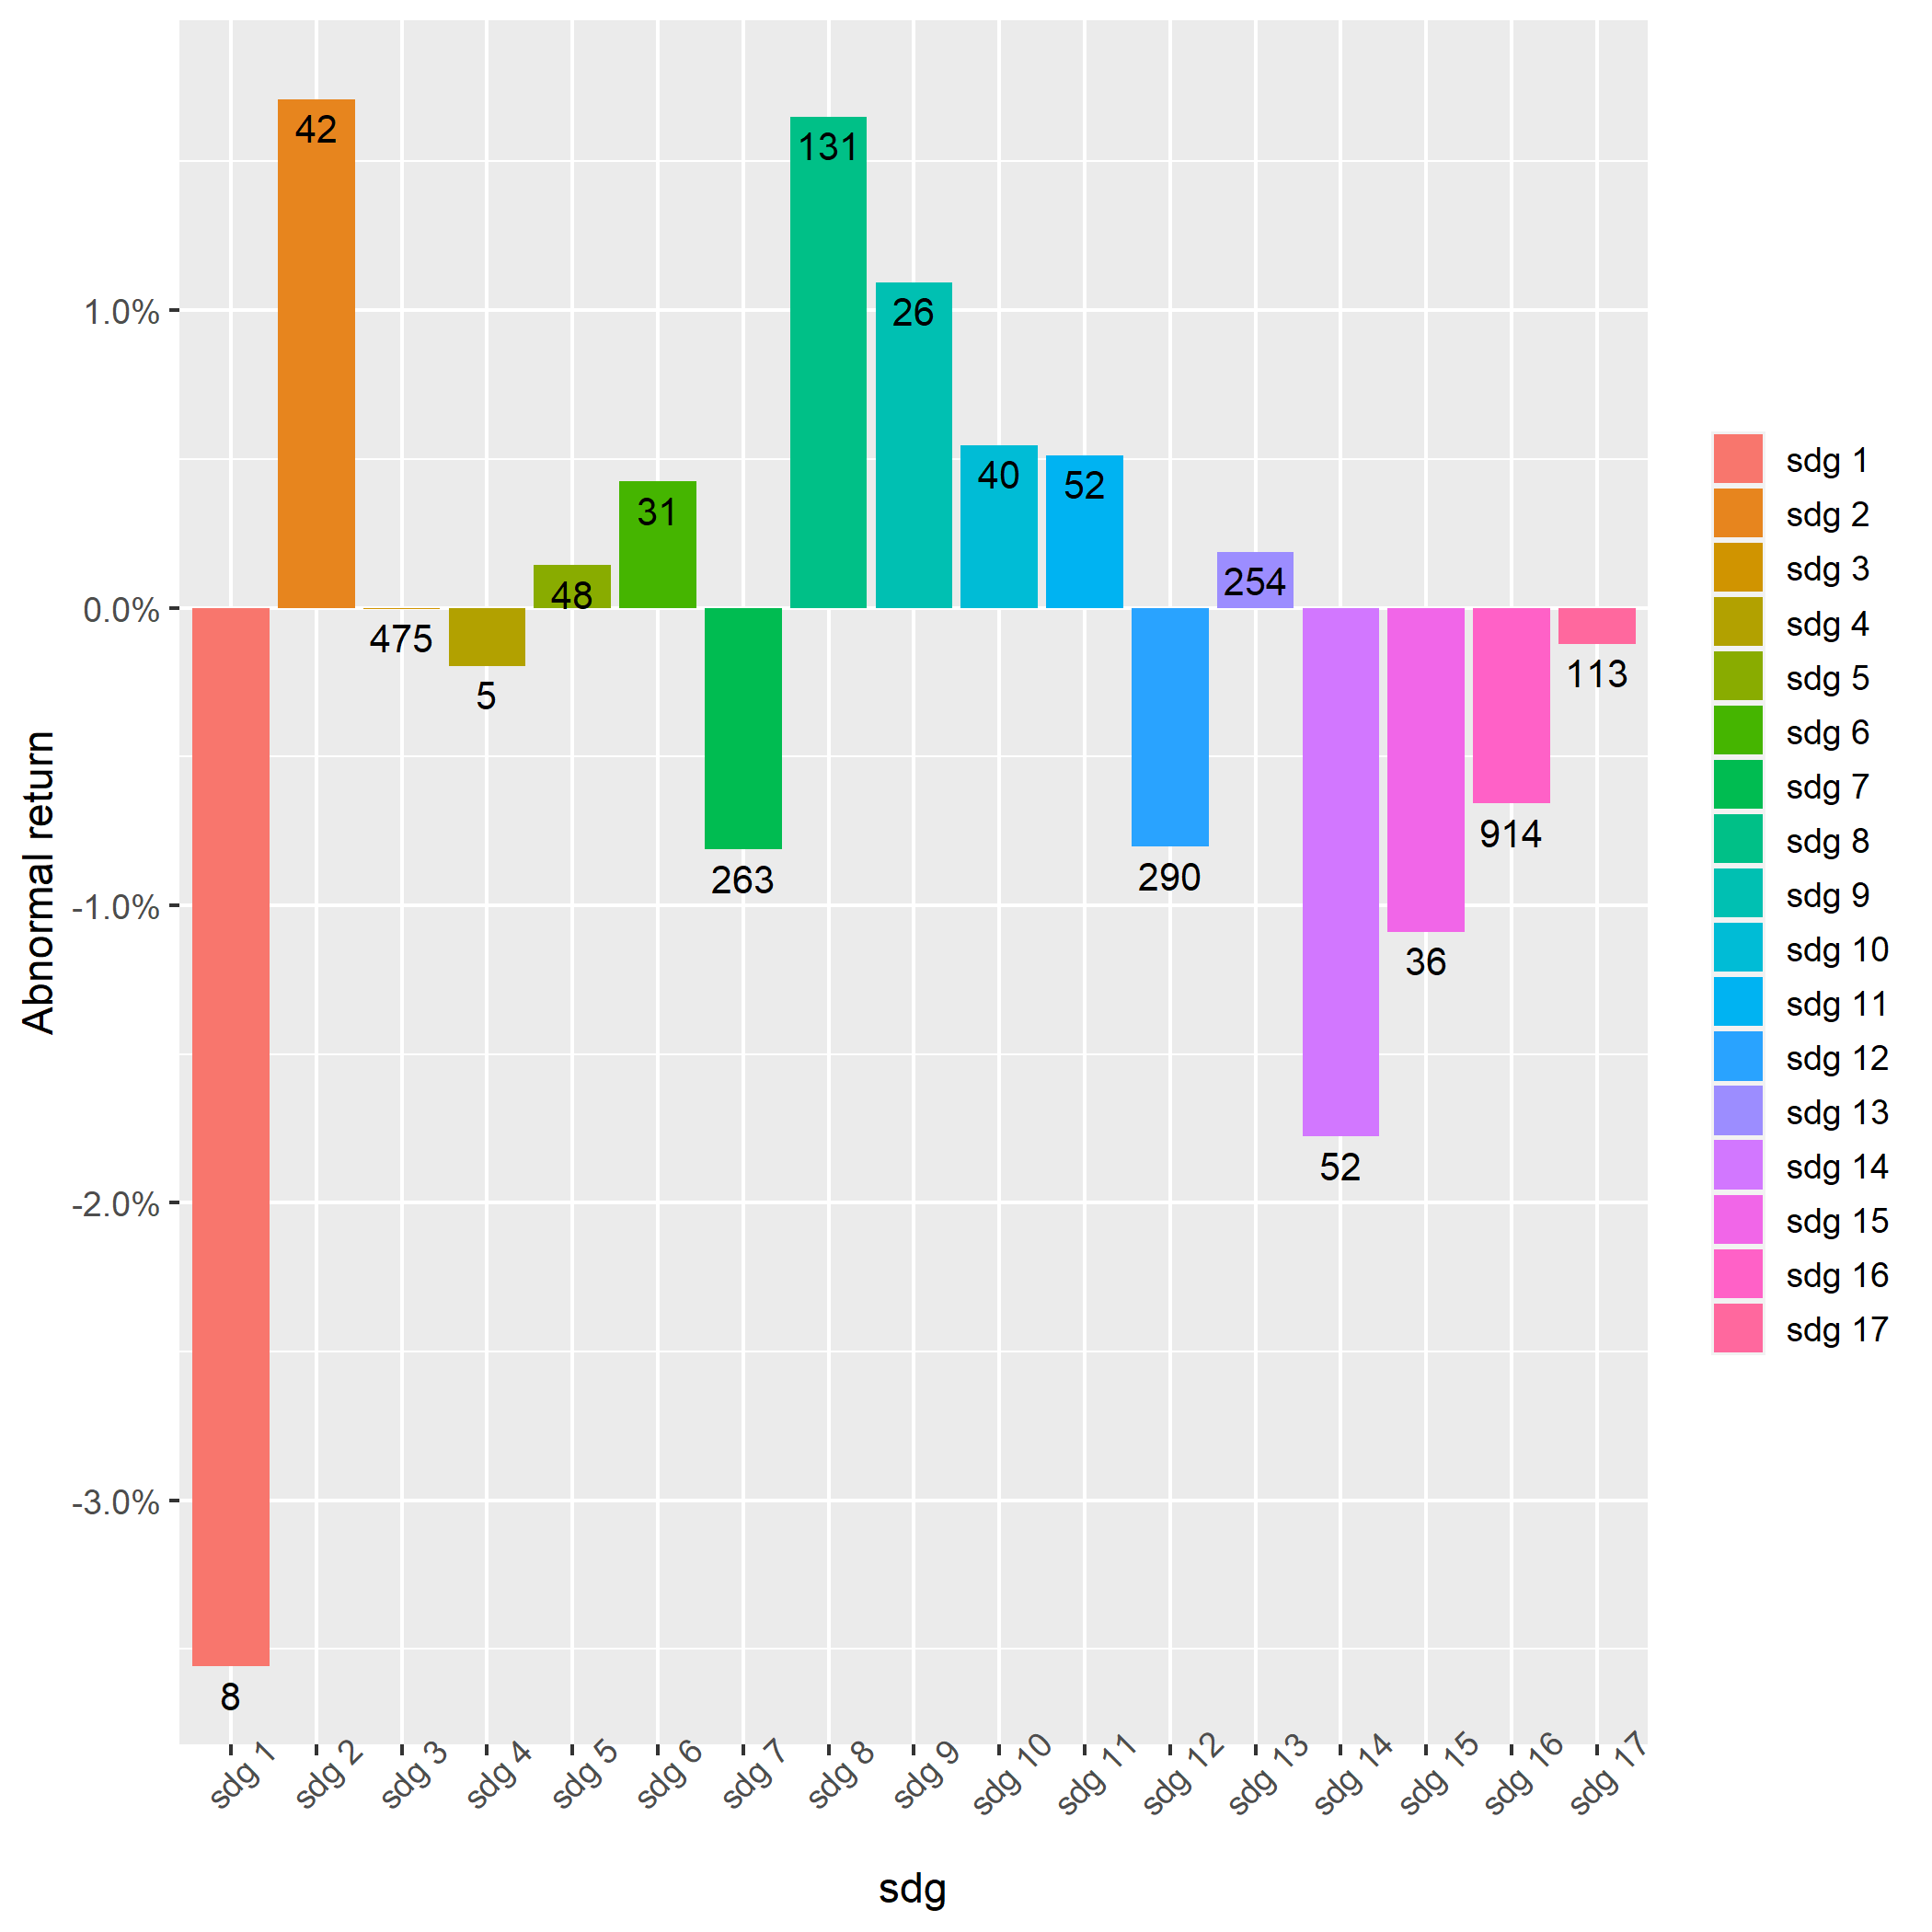
\includegraphics[scale=0.6]{Projekt/1.Figures analysis/ST_negative_sdg_bar.png}
    \caption*{\footnotesize The figure illustrates the AAR on $t = 0$ from negative news. The error bars represent the 95\% confidence intervals of the AAR.}
    \label{fig:ST_neg_bar_all}
\end{figure}

\begin{figure} [H]
    \centering
    \caption{AAR per SDG: positive news}
    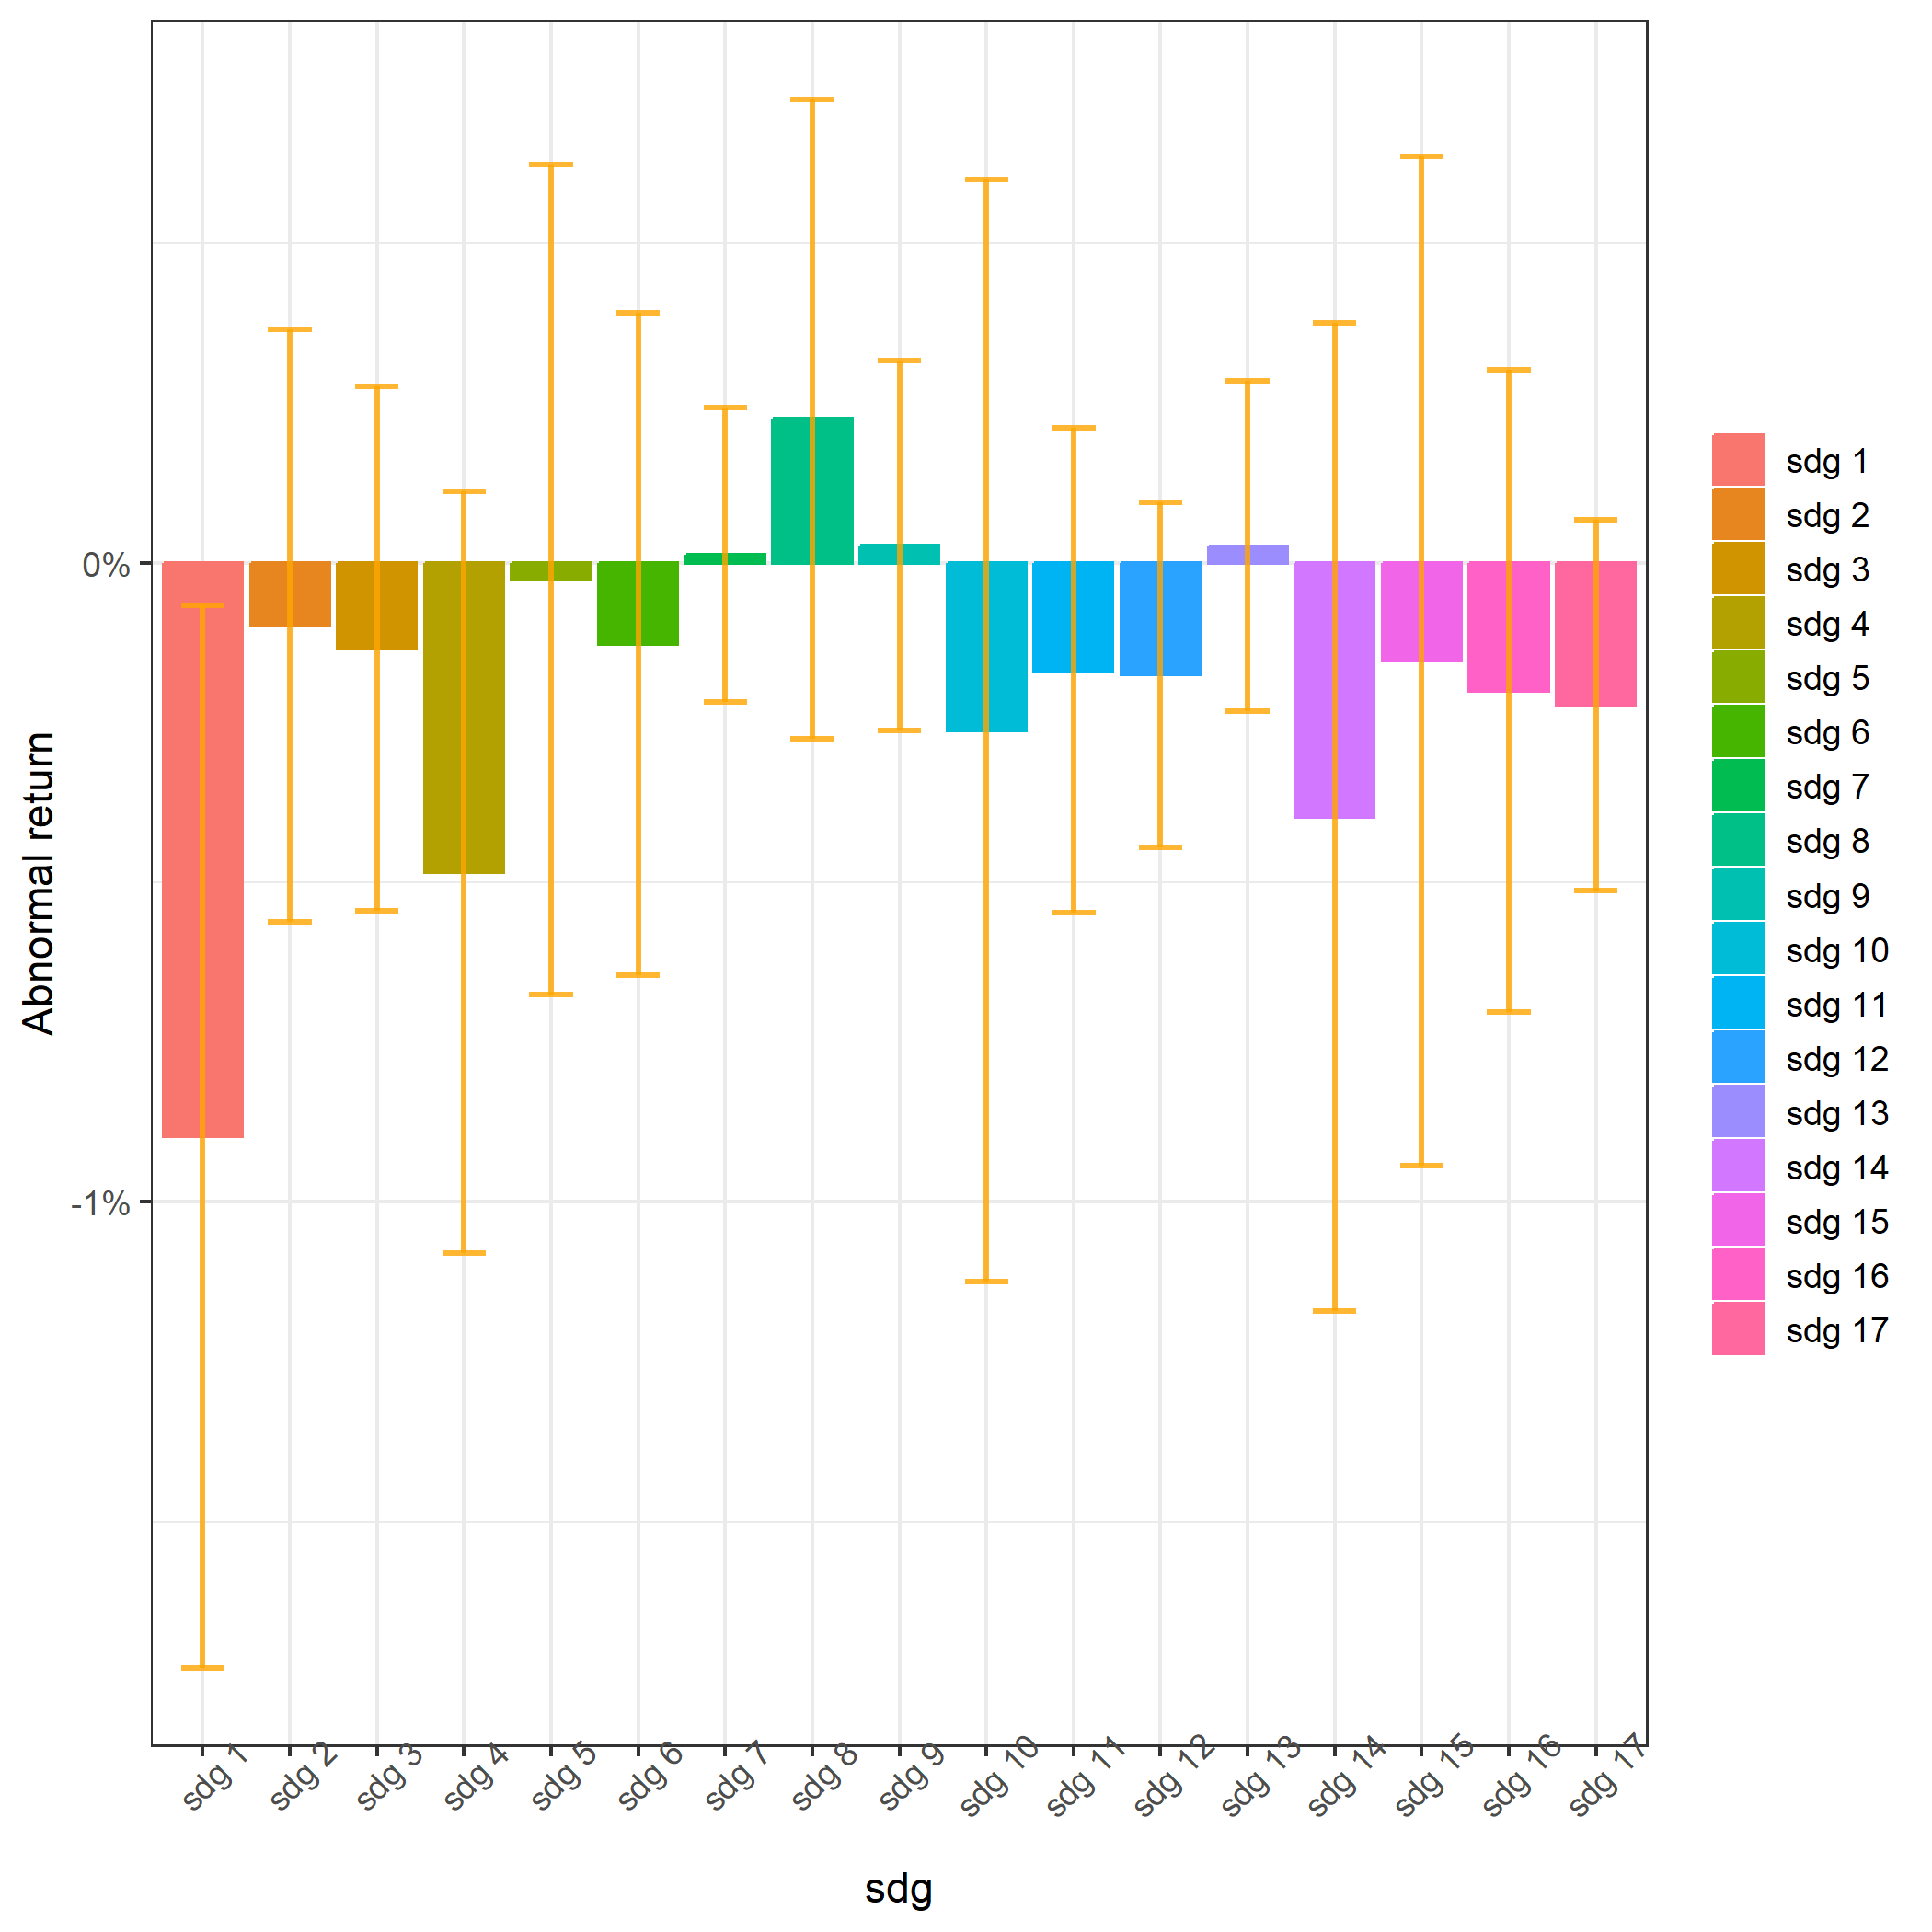
\includegraphics[scale=0.6]{Projekt/1.Figures analysis/ST_positive_sdg_bar.png}
    \caption*{\footnotesize The figure illustrates the AAR on $t = 0$ from positive news. The error bars represent the 95\% confidence intervals of the AAR.}
    \label{fig:ST_pos_bar_all}
\end{figure}




\subsection{Sensitivity analysis figures:}

\subsubsection{Short term}


\begin{table}[H]
\centering
\caption{AAR and CAAR (in \%) with new event rule (sd)} 
\begin{tabular}{lccccc}
  \hline  \hline
  & \multicolumn{2}{c}{Positive} &  & \multicolumn{2}{c}{Negative}\\ \cline{2-3} \cline{5-6}  
  & 2 sd & 3 sd & & 2 sd & 3 sd   \\   
 \hline
$AAR_{t=0}$ & $\underset{(0.875)}{0.051}$ & $\underset{(-0.278)}{-0.022}$ & & $\underset{(-3.409)}{-0.522^{***}}$ & $\underset{(-3.024)}{-0.617^{***}}$ \\ 
$CAAR_{[-2;+2]}$  & $\underset{(0.283)}{0.031}$  & $\underset{(0.631)}{0.089}$ & & $\underset{(-3.66)}{-0.714^{***}}$ & $\underset{(-2.648)}{-0.657^{***}}$ \\ 
$CAAR_{[-5;+5]}$  & $\underset{(1.197)}{0.195}$  & $\underset{(1.350)}{0.290}$ & &$\underset{(-3.56)}{-0.902^{***}}$ & $\underset{(-2.782)}{-0.867^{***}}$ \\ 
$CAAR_{[-10;+10]}$  & $\underset{(-0.168)}{-0.035}$  & $\underset{(-0.062)}{-0.018}$ &  & $\underset{(-1.886)}{-0.652^{*}}$ & $\underset{(-1.686)}{-0.697^{*}}$ \\ 
N & 1845 & 1078 & & 648 & 451  \\
   \hline \hline
   \multicolumn{6}{p{12cm}}{ \footnotesize $^* \; p\; <\; 0.1$, $ ^{**} \; p\; <\; 0.05$, $ ^{***} \; p\; <\; 0.01$  } \\
   \multicolumn{6}{p{13cm}}{\footnotesize The table shows the CAAR associated with positive and negative news over an event window of 5, 10, and 21 days surrounding the event date along with the AAR on $t=0$. The models are split on the requirement rule for included events (2 or 3 sd).} \\
   \hline
\end{tabular}
\label{tab:ST_sensitivity}
\end{table}


\begin{table}[H]
\centering
\caption{AAR and CAAR (in \%) with equally weighted returns} 
\begin{tabular}{lcccc}
  \hline  \hline
  & \multicolumn{1}{c}{Positive} &  \multicolumn{1}{c}{Negative}\\  
 \hline
$AAR_{t=0}$ &  $\underset{(0.634)}{0.045}$ & $\underset{(-3.509)}{-0.378^{***}}$ \\  
$CAAR_{[-5;+5]}$  & $\underset{(-1.233)}{-0.258}$ & $\underset{(-4.4255)}{-0.858^{***}}$ \\ 
$CAAR_{[-10;+10]}$    & $\underset{(-0.452)}{-0.128 }$ & $\underset{(-3.012)}{-0.822^{***}}$ \\ 
   \hline \hline
   \multicolumn{3}{p{10cm}}{ \footnotesize $^* \; p\; <\; 0.1$, $ ^{**} \; p\; <\; 0.05$, $ ^{***} \; p\; <\; 0.01$  } \\
   \multicolumn{3}{p{10cm}}{\footnotesize The tables shows the CAAR associated with positive and negative news over an event window of 5, 10, and 21 days surrounding the event date along with the AAR on $t=0$. The models are split on the requirement rule for included events (2 or 3 sd).} \\
   \hline
\end{tabular}
\label{tab:ST_sensitivity_weights}
\end{table}


\begin{figure} [H]
    \centering
    \caption{Positive news: event identification rule}
    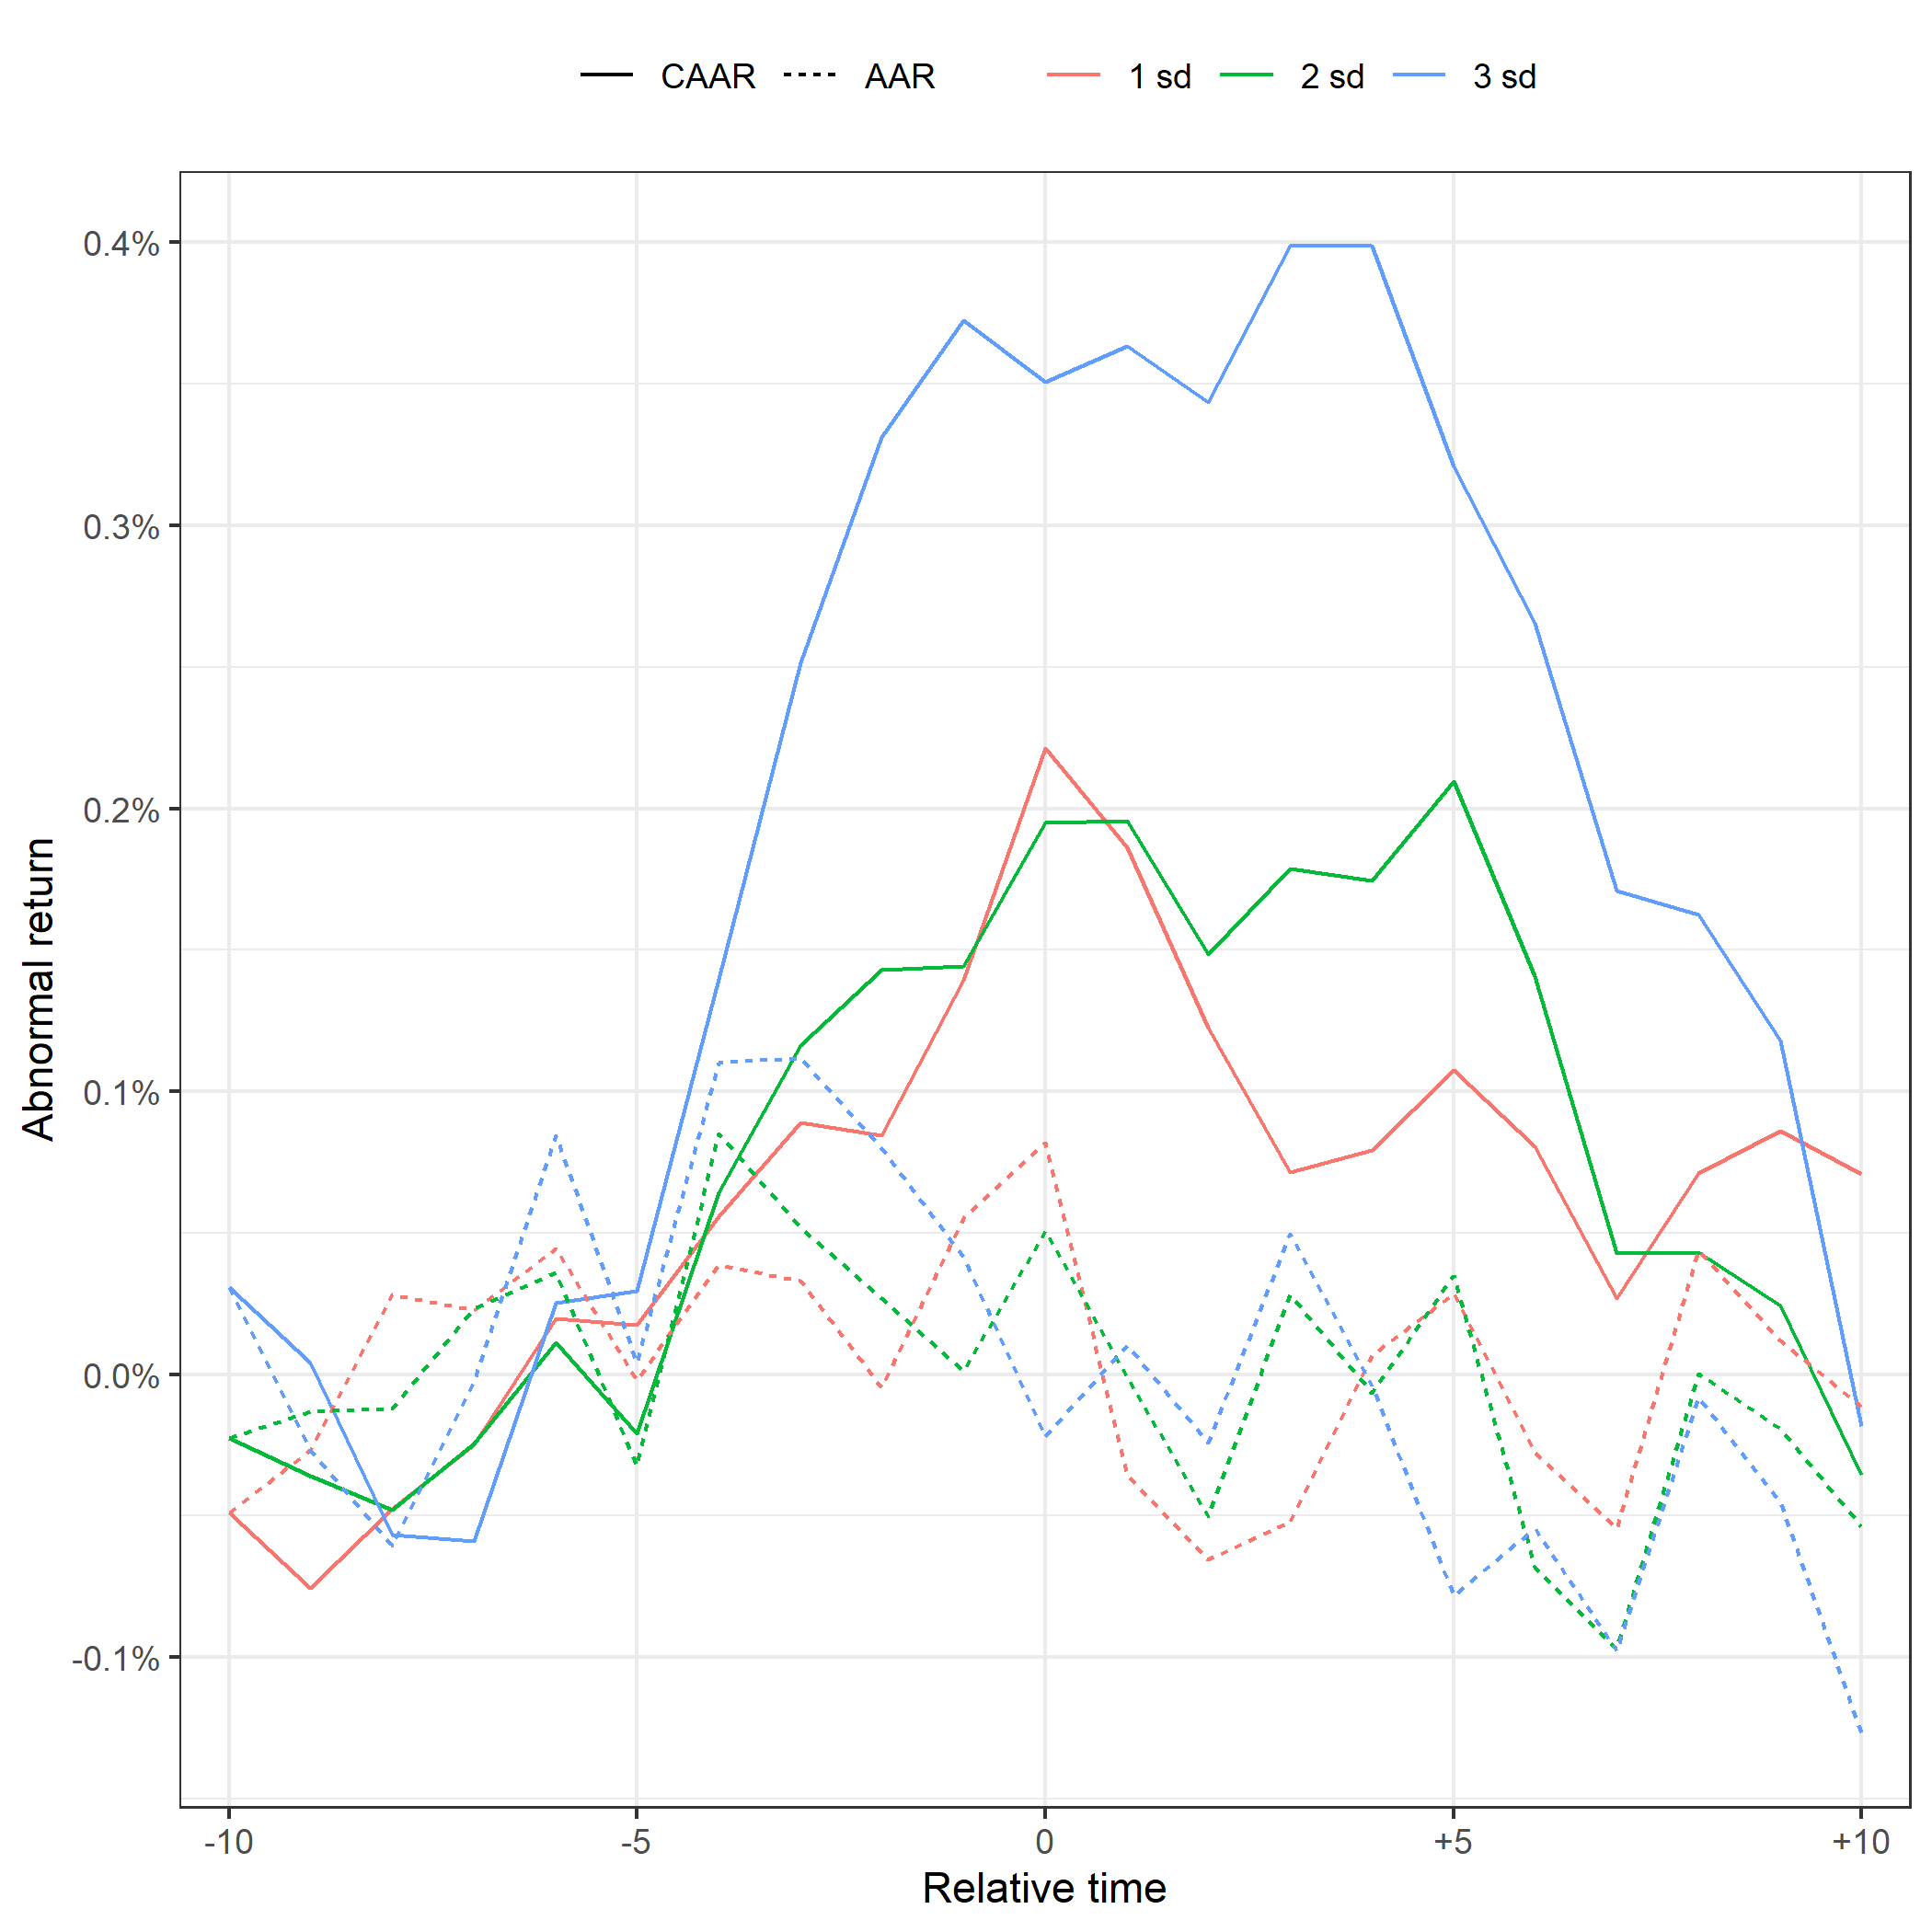
\includegraphics[scale=0.6]{Projekt/1.Figures analysis/ST_positive_sensitivity.png}
     \caption*{\footnotesize The figure illustrates the average abnormal return (AAR) and cumulative AAR (CAAR) around the event date (t = 0) of negative news. The figure illustrates the average abnormal return (AAR) and cumulative AAR (CAAR) around the event date (t = 0) of negative news. The various colors represent whether the event identification rule was based on 1, 2, or 3 standard errors. }
    \label{fig:ST_pos_sensi_sd}
\end{figure} 

\begin{figure} [H]
    \centering
    \caption{Positive news: Value vs. Equal weights}
    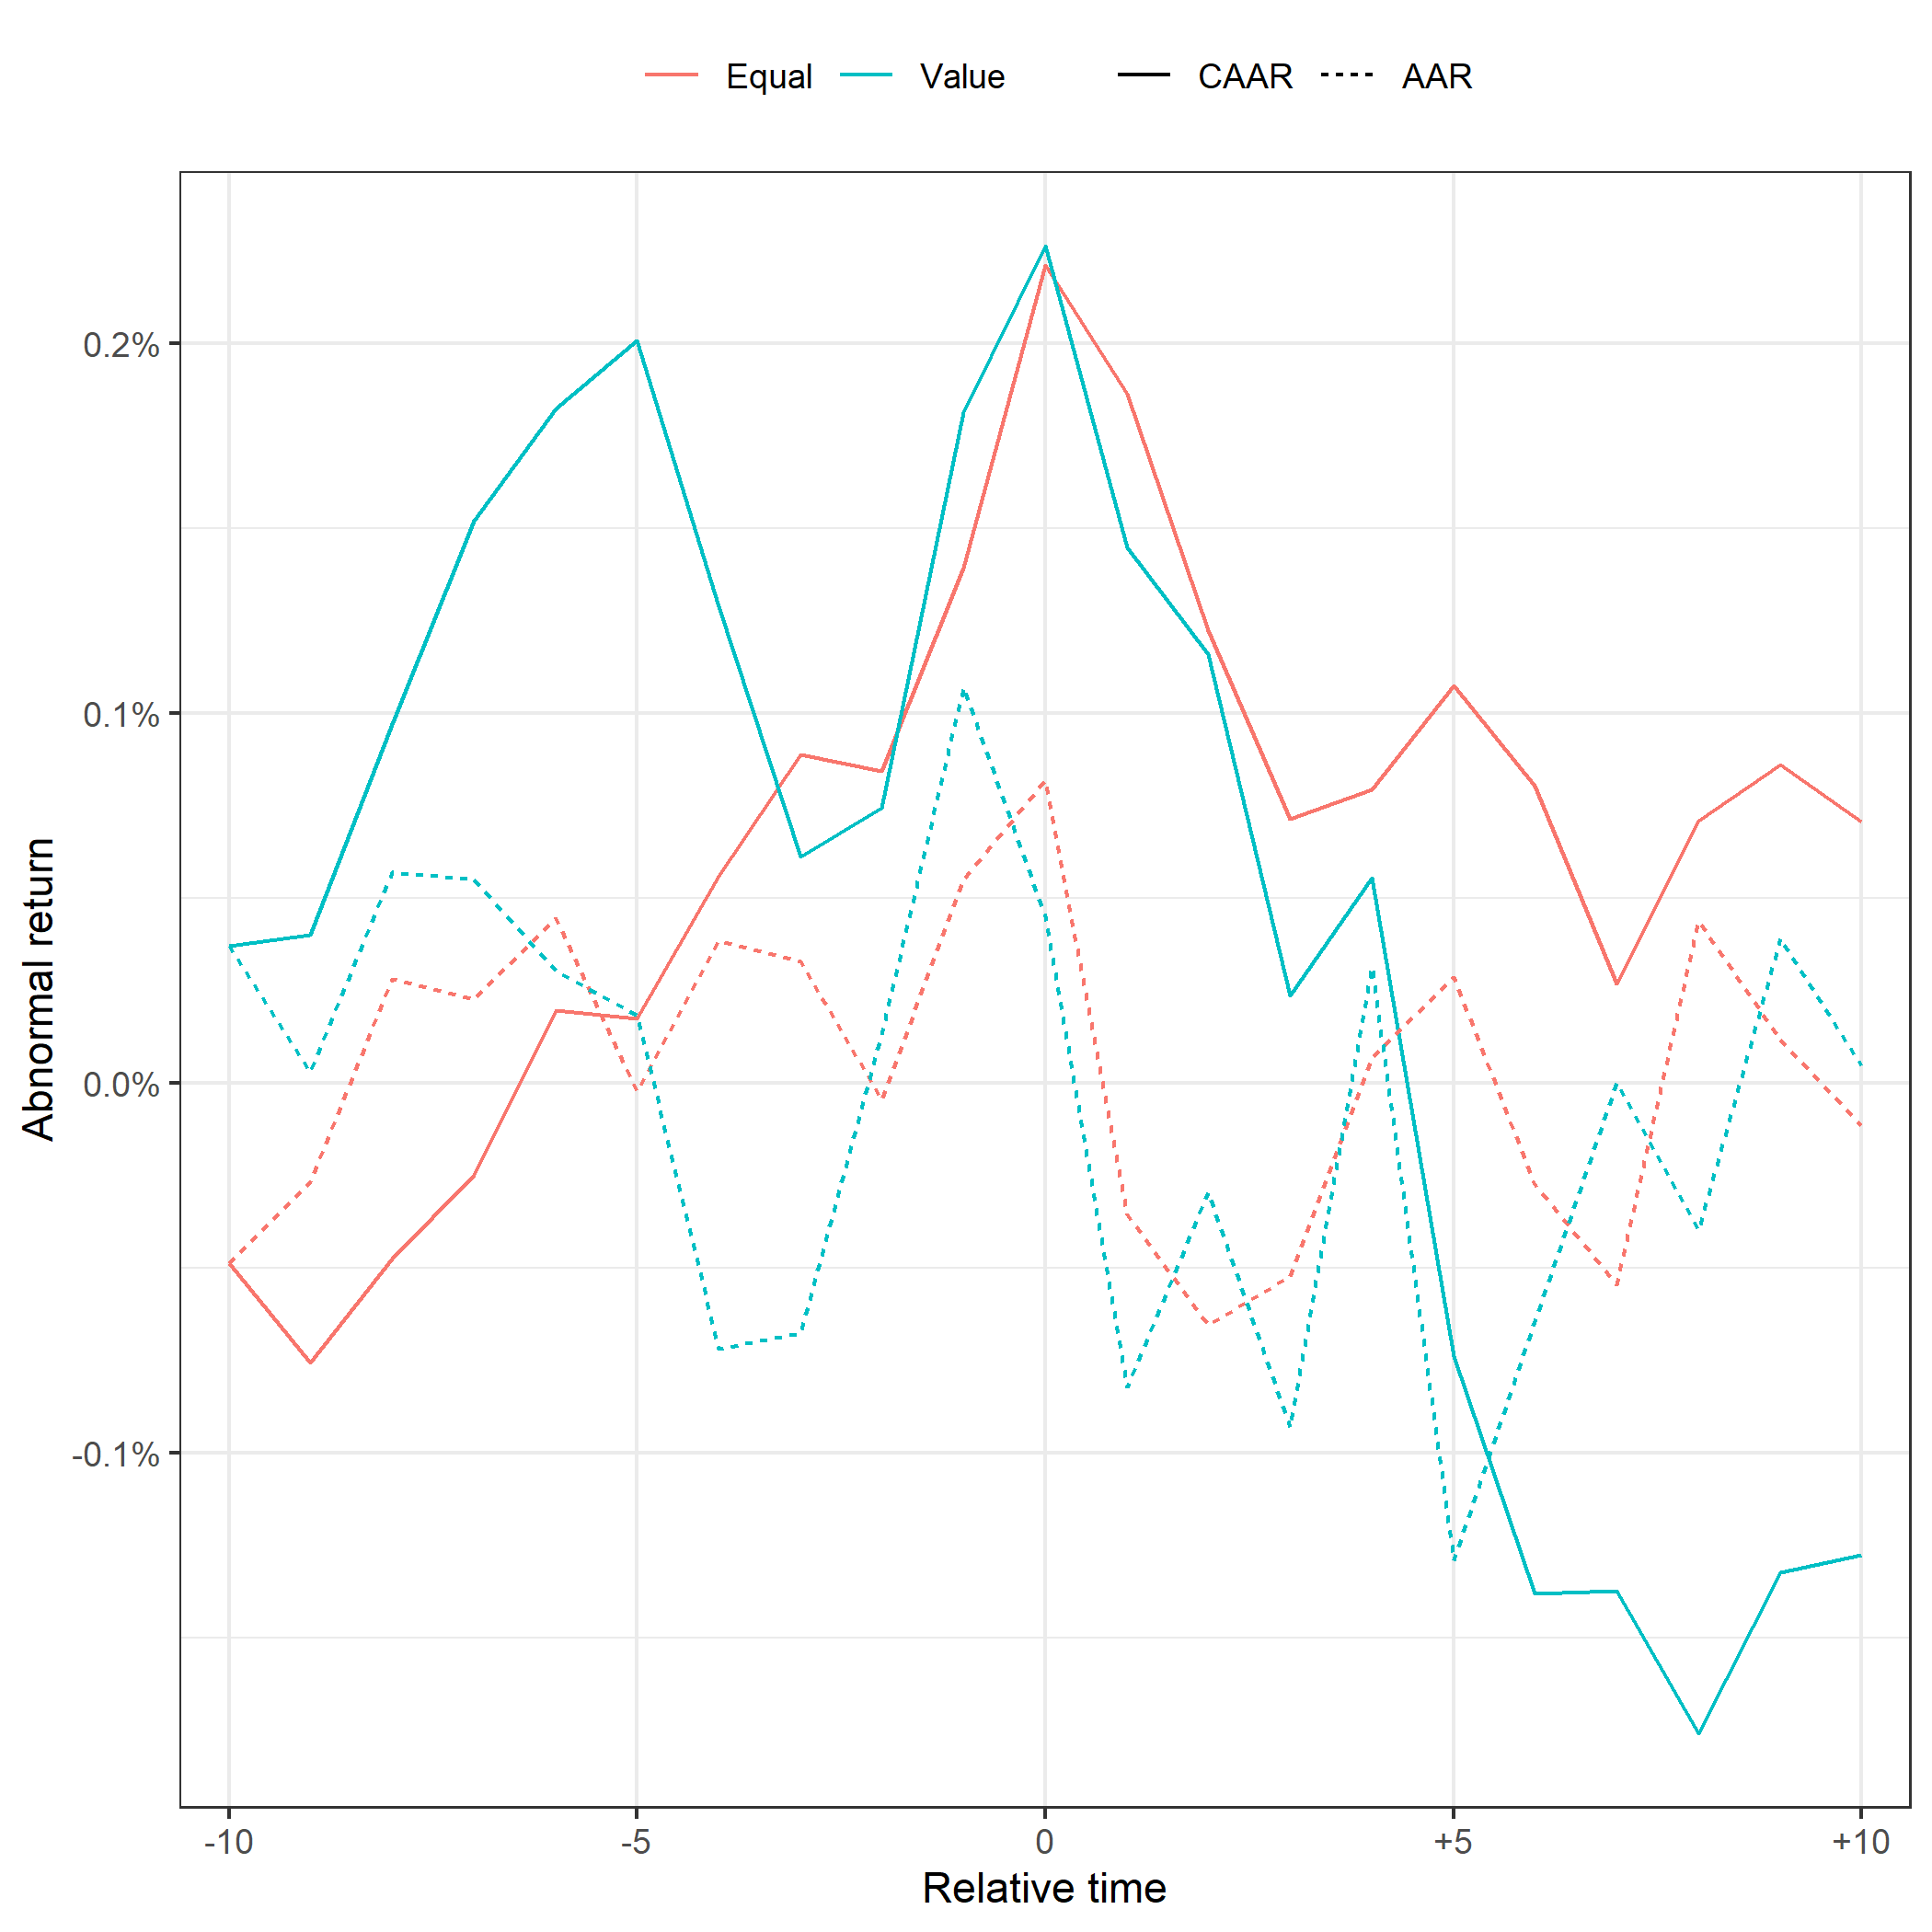
\includegraphics[scale=0.6]{Projekt/1.Figures analysis/ST_positive_sensitivity_weight.png}
     \caption*{\footnotesize The figure illustrates the average abnormal return (AAR) and cumulative AAR (CAAR) around the event date (t = 0) of positive news. The blue lines are returns calculated from an equally weighted portfolio, while the weights of the red lines are based on market capitalization. }
    \label{fig:ST_pos_sensitivity_weights}
\end{figure} 

\subsubsection{Long term}


\setlength{\tabcolsep}{15pt}
\begin{table}[]
\small
\centering
\caption{Fama-French five-factor model alpha from positive news with equal weights} 
\begin{tabular}{ccccccc}
\hline \hline \\ 
 &     &  &    1 SD  &  2 SD  &  3 SD  &  \\ \cline{4-6} 
& & & \multicolumn{3}{c}{ T = 1} & \\ \cline{2-6}
& Alpha (\%)  &  & $ -0.004$  & $-0.000$  & $-0.006$ &  \\
& t-value &  & -1.55 & -0.27  & -1.48 & \\
& & & \multicolumn{3}{c}{ T = 4} & \\ \cline{2-6}
& Alpha (\%)  &  & $ -0.003^{*}$  & $-0.001^{***}$  &  $-005^{**}$ & \\
& t-value & & -1.77  & -0.75 & -227 & \\
& & & \multicolumn{3}{c}{ T = 8} & \\ \cline{2-6}
& Alpha (\%)  &  & $ -0.003^{***}$   & $-0.003^{**}$  & $-0.005^{**}$ &  \\
& t-value &  & -2.98  & -2.45 & 3.51 & \\
&  & & \multicolumn{3}{c}{ T = 12} & \\ \cline{2-6}
& Alpha (\%)  &  & $ -0.004^{***}$  & $-0.003^{**}$  & $-0.003^{**}$ &  \\
& t-value &  & -3.02  & -2.66 & -1.12 & \\
\hline \hline
 \multicolumn{7}{l}{ \footnotesize $^* \; p\; <\; 0.1$, $ ^{**} \; p\; <\; 0.05$, $ ^{***} \; p\; <\; 0.01$  } \\
 \multicolumn{7}{p{11.5cm}}{ \footnotesize Alpha is the WLS-regression intercept (in \%) of the Fama-French 3-factor model, displayed along with the corresponding t-value. N is the average amount of firms included in the portfolio each month, and T is the portfolio holding period. The threshold for event firms to be included in the portfolio is either 1,2 or 3 "SD" (standard deviations) larger than the mean.}  \\ 
\end{tabular}
\label{tab: FF5_pos_equalW}
\end{table}


\setlength{\tabcolsep}{15pt}
\begin{table}[H]
\small
\centering
\caption{FF-5 model alpha from positive news with altered event identification rule } 
\begin{tabular}{ccc}
\hline \hline \\ 
&  2 SD  &  3 SD   \\ \cline{2-3} 
 \multicolumn{2}{c}{ T = 1}  \\ \hline
 Alpha (\%) & 0.04  & -0.37   \\
 t-value & 0.11  & -0.74  \\
 \multicolumn{2}{c}{ T = 4}  \\ \hline
 Alpha (\%)  & 0.03  &  -0.07  \\
 t-value  & 0.13  & -0.23  \\
 \multicolumn{2}{c}{ T = 8}  \\ \hline
 Alpha (\%) & -0.01  & 0.04   \\
 t-value & -0.15 & 0.18  \\
 \multicolumn{2}{c}{ T = 12}  \\ \hline
 Alpha (\%) & 0.13  & 0.23   \\
 t-value & 1.09 & 1.35  \\
 \hline \hline
 \multicolumn{3}{l}{ \footnotesize $^* \; p\; <\; 0.1$, $ ^{**} \; p\; <\; 0.05$, $ ^{***} \; p\; <\; 0.01$  } \\
 \multicolumn{3}{p{5cm}}{ \footnotesize Alpha is the WLS-regression intercept (in \%) of the Fama-French 5-factor model, displayed along with the corresponding t-value. N is the average amount of firms included in the portfolio each month, and T is the portfolio holding period. The threshold for event firms to be included in the portfolio is either 1,2 or 3 standard deviations (SD) larger than the mean.}  \\ 
\end{tabular}
\label{tab: FF5_pos}
\end{table}

\pagebreak



\end{document}